%Version 3 December 2023
% See section 11 of the User Manual for version history
%
%%%%%%%%%%%%%%%%%%%%%%%%%%%%%%%%%%%%%%%%%%%%%%%%%%%%%%%%%%%%%%%%%%%%%%
%%                                                                 %%
%% Please do not use \input{...} to include other tex files.       %%
%% Submit your LaTeX manuscript as one .tex document.              %%
%%                                                                 %%
%% All additional figures and files should be attached             %%
%% separately and not embedded in the \TeX\ document itself.       %%
%%                                                                 %%
%%%%%%%%%%%%%%%%%%%%%%%%%%%%%%%%%%%%%%%%%%%%%%%%%%%%%%%%%%%%%%%%%%%%%

%%\documentclass[referee,sn-basic]{sn-jnl}% referee option is meant for double line spacing

%%=======================================================%%
%% to print line numbers in the margin use lineno option %%
%%=======================================================%%

%%\documentclass[lineno,sn-basic]{sn-jnl}% Basic Springer Nature Reference Style/Chemistry Reference Style

%%======================================================%%
%% to compile with pdflatex/xelatex use pdflatex option %%
%%======================================================%%

%%\documentclass[pdflatex,sn-basic]{sn-jnl}% Basic Springer Nature Reference Style/Chemistry Reference Style


%%Note: the following reference styles support Namedate and Numbered referencing. By default the style follows the most common style. To switch between the options you can add or remove “Numbered” in the optional parenthesis. 
%%The option is available for: sn-basic.bst, sn-vancouver.bst, sn-chicago.bst%  
 
\documentclass[pdflatex,sn-nature]{sn-jnl}% Style for submissions to Nature Portfolio journals
%%\documentclass[pdflatex,sn-basic]{sn-jnl}% Basic Springer Nature Reference Style/Chemistry Reference Style
%%\documentclass[pdflatex,sn-mathphys-num]{sn-jnl}% Math and Physical Sciences Numbered Reference Style 
%%\documentclass[pdflatex,sn-mathphys-ay]{sn-jnl}% Math and Physical Sciences Author Year Reference Style
%%\documentclass[pdflatex,sn-aps]{sn-jnl}% American Physical Society (APS) Reference Style
%%\documentclass[pdflatex,sn-vancouver,Numbered]{sn-jnl}% Vancouver Reference Style
%%\documentclass[pdflatex,sn-apa]{sn-jnl}% APA Reference Style 
%%\documentclass[pdflatex,sn-chicago]{sn-jnl}% Chicago-based Humanities Reference Style

%%%% Standard Packages
%%<additional latex packages if required can be included here>

\usepackage{graphicx}%
\usepackage{multirow}%
\usepackage{amsmath,amssymb,amsfonts}%
\usepackage{amsthm}%
\usepackage{mathrsfs}%
\usepackage[title]{appendix}%
\usepackage{xcolor}%
\usepackage{color, colortbl}
\usepackage{textcomp}%
\usepackage{manyfoot}%
\usepackage{booktabs}%
\usepackage{algorithm}%
\usepackage{algorithmicx}%
\usepackage{algpseudocode}%
\usepackage{listings}%
\usepackage{comment}
\usepackage{newtxtext,newtxmath}
\usepackage[utf8]{inputenc}
\usepackage{newfloat}

% Define a new floating environment for Extended Data Figures
\DeclareFloatingEnvironment[
fileext=loe,
placement={!ht},
name={Extended Data Fig.}
]{extfigure}
\DeclareUnicodeCharacter{2009}{\,}


%% as per the requirement new theorem styles can be included as shown below
%\theoremstyle{thmstyleone}%
%\newtheorem{theorem}{Theorem}%  meant for continuous numbers
%%\newtheorem{theorem}{Theorem}[section]% meant for sectionwise numbers
%% optional argument [theorem] produces theorem numbering sequence instead of independent numbers for Proposition
%\newtheorem{proposition}[theorem]{Proposition}% 
%%\newtheorem{proposition}{Proposition}% to get separate numbers for theorem and proposition etc.

%%\theoremstyle{thmstyletwo}%
%\newtheorem{example}{Example}%
%\newtheorem{remark}{Remark}%

%\theoremstyle{thmstylethree}%
%\newtheorem{definition}{Definition}%

%\raggedbottom
%%\unnumbered% uncomment this for unnumbered level heads

\begin{document}
%titulo 75 caracteres contando espacios
\title[Article Title]{Bayesian evidence for asymmetric activation of P2X2 receptors}
\author*[1]{\fnm{Luciano} \sur{Moffatt}}\email{lmoffatt@qi.fcen.uba.ar}
\author[2]{\fnm{Gustavo} \sur{Pierdominici-Sottile}}\email{gsottile@unq.edu.ar}
%\equalcont{These authors contributed equally to this work.}

%\author[1,2]{\fnm{Third} \sur{Author}}\email{iiiauthor@gmail.com}
%\equalcont{These authors contributed equally to this work.}

\affil*[1]{\orgdiv{Instituto de Qu\'{i}mica F\'{i}sica de los Materiales, Medio Ambiente y Energ\'{i}a}, \orgname{  Consejo Nacional de Investigaciones Científicas y T\'{e}cnicas}, \orgname{Universidad de Buenos Aires} , \city{Buenos Aires}, \postcode{1428},  \country{Argentina}}

\affil[2]{\orgdiv{Departamento de Ciencia y Tecnolog\'{i}a, 
  Consejo Nacional de Investigaciones Científicas y T\'{e}cnicas} \orgname{Universidad Nacional de Quilmes}, \orgaddress{\street{S\'{a}enz Pe\~{n}a 352}, \city{Bernal}, \postcode{B1876BXD}, \state{Buenos Aires}, \country{Argentina}}}

%\affil[3]{\orgdiv{Department}, \orgname{Organization}, \orgaddress{\street{Street}, \city{City}, \postcode{610101}, \state{State}, \country{Country}}}


\abstract{
Ligand‐gated ion channel activation is central to cellular signal transduction, influencing processes from neurotransmission to immune responses\cite{Changeux1984AcetylcholineRA,UNWIN199331,Lemoine2012,galligan2002ligand,feske2012ion}. ATP‐activated P2X receptors, with their minimalist trimeric structure, serve as an excellent model for exploring allosteric regulation\cite{Nicke1998P2X1AP,Sattler2020UnravellingTI,abierta_p2x,Moffatt_hume}. Although structural studies have defined their closed and open states\cite{abierta_p2x,cerrada_p2x}, the precise sequence of ATP‐driven conformational changes and the role of subunit‐specific dynamics remain unclear.

Here, we show that the activation kinetics of P2X2 receptors are reproduced by an asymmetric coupling mechanism, whereby ATP binding induces the rotation of individual subunits and a saturating increase in conductance. Combining a novel Bayesian analysis of time‐averaged macroscopic currents with single-bound P2X molecular dynamics simulations, we demonstrate that ATP binding stabilizes and lowers the energetic barrier for partial rotation of the subunit on the left of the binding site while minimally affecting the right. This induced rotation, in turn, increases the barrier for ATP binding at the left‐facing site, accounting for the observed negative cooperativity and preventing unliganded rotation that would lead to premature inactivation.

Our findings suggest that tunable activation barriers represent a general strategy for stabilizing ion channels and signaling proteins in dynamic cellular environments, with implications for drug design in chronic pain and inflammation.
}



\keywords{Bayesian Analysis, P2X receptors, Activation kinetics, Energy barrier modulation}

\maketitle
\section{Introduction}
Ligand‐gated ion channels (LGICs) are multimeric membrane proteins that convert chemical signals into electrical responses by coupling ligand binding to the opening of an ion‐conducting pore \cite{Changeux1984AcetylcholineRA,UNWIN199331,Lemoine2012,galligan2002ligand,feske2012ion}. By transforming the energy of ligand binding into conformational changes that modulate pore conductance, these receptors underpin fast synaptic transmission, muscle contraction, and other essential physiological processes \cite{nakanishi1994metabotropic,greengard2001neurobiology,burnstock2007physiology}. Among LGICs, ATP‐activated P2X receptors are particularly attractive as model systems due to their minimalist trimeric architecture, intersubunit ATP‐binding sites \cite{MarquezKlaka2007IdentificationOA}, and the availability of high‐resolution structures for both the closed \cite{cerrada_p2x} and open \cite{abierta_p2x} states.

A comprehensive understanding of P2X receptor activation requires a framework that links the molecular mechanisms underlying the kinetic variability observed in experiments with the structural insights accessible via MD simulations. While single‐channel Markov models capture the stochastic behavior of individual channels \cite{properties_single_channe}, macroscopic current fluctuations reflect the collective dynamics of many channels \cite{Moffatt_hume}. Historically, a disconnect has persisted between kinetic schemes derived from single‐channel data and the molecular mechanisms governing channel activation \cite{abierta_p2x}. The allosteric Monod–Wyman–Changeux (MWC) model \cite{Changeux1984AcetylcholineRA} has provided a thermodynamic framework to reconcile these aspects, as demonstrated in studies on BK channels \cite{Horrigan2002CouplingBV} and, more recently, purinergic receptors \cite{Moffatt_hume,Sattler2020UnravellingTI}.

Here, we address this challenge with three complementary advances. First, we introduce \textit{MacroIR}, a Bayesian framework that analyzes time‐averaged macroscopic currents while preserving temporal correlations and enabling rapid evaluation of complex kinetic schemes. Unlike previous methods \cite{Munch2022}, \textit{MacroIR} explicitly incorporates the system state at both the onset and conclusion of the averaging interval. Second, we develop conformational models that directly relate kinetic transitions to physical subunit rotations, eliminating the need for hypothetical intermediates (e.g., the flip state \cite{Moffatt_hume,jiang2012intermediate,browne2013p2x}). Third, we employ Molecular Dynamics (MD) simulations of single‐bound P2X receptors to elucidate the asymmetry in subunit fluctuations predicted by our models.

Together, these advances provide robust Bayesian evidence and MD support for kinetic asymmetry in P2X2 receptor activation, reveal modulation of the activation barrier that prevents premature inactivation, and offer a general blueprint for integrating kinetic data with structural mechanisms.

\section{Methods}\label{sec:methods}

In this section, we detail our Bayesian analysis framework, including the experimental data used to evaluate our approach, the kinetic schemes developed for prediction, the likelihood function quantifying predictive accuracy, and the algorithm for computing Bayesian evidence to compare alternative kinetic models and infer posterior parameter distributions. In addition, we describe how the conformational ensemble of the closed P2X receptor—docked with an ATP molecule—was sampled using Molecular Dynamics simulations.

\subsection{Bayesian Analysis}
\subsubsection{Why a Bayesian Approach?}
A Bayesian framework is ideally suited for analyzing macroscopic currents because it directly addresses the challenge of temporal autocorrelation—a consequence of successive observations on the same finite population of channels in a macropatch. Both the MacroR and MacroIR algorithms exploit this autocorrelation to extract detailed kinetic information by continuously updating our belief about the probability distribution over the possible kinetic states.

At each stage, these algorithms iteratively refine the posterior probability distribution—approximated as a normal distribution—to yield a dynamic, high-resolution estimate of the kinetic states. Notably, this process also produces a correlation matrix among the states of different channels. It is important to emphasize that this correlation does not imply a causal influence between neighboring channels; rather, it arises because the aggregate current reflects the sum of individual channel contributions, thereby coupling the information on channel states in the observer’s inference. In this sense, the phenomenon is reminiscent of quantum entanglement, where correlations become apparent only after measurement.
\subsubsection{Objective of the Bayesian Analysis}
The primary objective of our Bayesian analysis is to extract mechanistic insights from the stochastic fluctuations observed in macrocurrents. We achieve this through two complementary strategies:

\begin{enumerate}[label=\textbf{\arabic*.}]
    \item \textbf{Comparison of Alternative Molecular Mechanisms and Kinetic Schemes.}  
    We translate each proposed molecular mechanism into a corresponding kinetic scheme. In addition, we include previously proposed kinetic schemes where the underlying molecular mechanism remains ambiguous. Bayesian evidence for each alternative is computed using our MCMC framework, and the kinetic schemes that yield the highest evidence are interpreted as having the strongest support from the experimental data. It is important to note that this analysis does not prove that a particular molecular mechanism is occurring; rather, it facilitates selection among a set of plausible alternatives. Definitive validation is achievable only when the set of alternatives encompasses all logically possible options.
    
    \item \textbf{Parameter Analysis of the Most Probable Kinetic Scheme.}  
    In parallel with model comparison, we perform a detailed analysis of the parameters within the most probable kinetic scheme. In particular, the examination of kinetic coupling enables us to assess whether modulation of kinetic barriers occurs beyond simple regulation of equilibrium constants. Furthermore, evaluating the dependency of the current on the number of rotated subunits provides critical insight into how subunit rotation influences pore permeability.
\end{enumerate}

Collectively, these approaches provide a robust framework for deriving mechanistic interpretations from macroscopic current recordings and for elucidating the kinetics of P2X2 receptor activation.

\subsubsection{Likelihood Function and Model Parameters}
The likelihood function defines the probability of observing the averaged recorded macroscopic current at each time interval, given a specific kinetic model and its associated parameters. The model parameters are categorized into distinct groups based on their functional role:

\begin{itemize}
    \item \textbf{Kinetic Scheme Parameters:} Parameters that characterize the transitions between channel states, formulated either as state-based or allosteric schemes.
    \item \textbf{Channel Availability Model:} We modeled the evolution of the number of available channels over the course of the experiment by incorporating processes such as inactivation. In this model, two parameters are used: the total number of channels and the inactivation rate. Inactivation is represented as a distinct state that is irreversibly accessible from all other states at a uniform rate.
    \item \textbf{Conductance Model:} Parameters that define the single-channel conductance, including potential state-dependent variations. 
    \item \textbf{Measurement Noise Model:} A model that accounts for stochastic fluctuations in the recorded signal, capturing both white and pink noise components.
    \item \textbf{Baseline Current Estimation:} A parameter that quantifies the residual baseline current present in the recordings.
\end{itemize}


All model parameters have a direct physical or material interpretation, meaning they correspond to measurable or experimentally relevant quantities. This ensures that parameter estimates can be directly related to the underlying biological and experimental conditions.

\subsubsection{Prior Distribution}
For each model, we specify a prior distribution for every parameter. Rather than encoding detailed prior knowledge of purinergic receptor kinetics, our priors were designed to encompass a broad range of plausible kinetic models, constrained only by general considerations. In this way, we aimed to favor kinetic schemes that structurally reflect receptor dynamics.

Since all parameters are inherently positive, we assigned each a log$_{10}$-normal prior with a common variance of 2 in log-space, ensuring that the bulk of the probability mass spans roughly two orders of magnitude around the median. The medians of these priors were set to reasonable values, avoiding undue bias toward any particular model configuration. In cases where symmetry is present, such as when two parameters are interchangeable (e.g., right versus left coupling or in schemes 3 and 4, which incorporate two equivalent open states), one branch was assigned a median 10 times greater than its counterpart.

For the kinetic rate constants, we selected an intermediate value of 100 s$^{-1}$, while the association rate was set at 10 s$^{-1}$ mM$^{-1}$. The equilibrium allosteric couplings were assigned the following values: BF = 100, BG = 1, FG = 100, RB = 100, BR = 10, and RBR = 1. By contrast, all kinetic allosteric couplings were uniformly set to 1.

Additional priors were specified as follows. The number of channels was fixed at 4800, the inactivation rate was set to $10^{-5}$ s$^{-1}$, and the measurement noise was defined with parameters of $10^{-3}$ pA$\cdot$s for white noise and 5 pA for pink noise. The unitary current was set to 1 pA (measured at $-60$ mV). Moreover, the leakage current was fixed at $10^{-6}$ pA, the allosteric factor (which increases the current due to subunit rotation) was set to 100, and the basal current was specified as 1 pA.   

\subsubsection*{Likelihood}
The likelihood is defined below (Equation~\eqref{eq:macroIR_likelihood}). Note that MacroIR is an approximation, valid only within certain regimes. In our implementation, if the approximation is found to be invalid over a given interval, we employ the MacroINR algorithm for that interval. This logic is implemented in the function \texttt{Macror} (line 3576 of \texttt{qmodel.h}; \url{https://github.com/lmoffatt/macro_dr_submission}).


\subsection{Experimental Data: Outside-out Patch Recording}

The experimental dataset analyzed in this study was previously published in \textit{The Journal of General Physiology} \cite{Moffatt_hume} and is reexamined here to develop and validate our approach. Recordings were obtained from macro outside-out patches containing hundreds to thousands of P2X2 channels. These patches were exposed to 0.2-ms ATP pulses at concentrations of 0.1, 0.2, 0.5, 1, 2, and 10 mM delivered every 2 minutes, interspersed with 10-ms pulses of 1 mM ATP. The dataset is ideally suited for kinetic analysis due to the precise alignment of stimulus timing with channel responses, which were recorded directly from the patch. For complete experimental details—including solution compositions, recording conditions, and data acquisition protocols—please refer to the original publication \cite{Moffatt_hume}.

For kinetic analysis, we segmented the data as follows. The 1 s pre-pulse period was divided into 72 intervals of 13.7 ms and 10 intervals of 0.02 ms. During the ATP pulse, as well as 0.24 ms before,  the algorithm processed the raw data, whereas after the pulse the data were averaged over exponentially spaced intervals (approximately 10 points per decade). Additionally, for each 10-ms ATP pulse, one averaged sample  was retained from the second half of the pulse, corresponding to the equilibrium current. 

\subsection{Kinetic Models Under Test}

We evaluated 11 kinetic models, including seven previously described by Moffatt and Hume \cite{Moffatt_hume} and four new models introduced in this study. These models can be classified  into three distinct categories: \textbf{state models}, which describe receptor kinetics without explicitly incorporating allosteric interactions; \textbf{allosteric models}, which introduce modulations between specific transitions without an explicit structural correspondence; and \textbf{conformational models}, which explicitly map kinetic transitions onto physical structural rearrangements.

\subsubsection{Previously Established Models}

The seven previously established models represent progressively complex descriptions of receptor activation:

\textbf{State Models:}  
- \textit{Scheme I}: A Minimal linear scheme for a homotrimeric channel in which all binding sites must be occupied before channel opening can occur.  
- \textit{Scheme II}: Extends Scheme I by introducing an intermediate "flipped" state (a hypothesized intermediate conformational state preceding opening) between the fully bound and open conformations, allowing for a sequential activation process.  
- \textit{Scheme III}: Preferred scheme on a single channel study \cite{properties_single_channe}, this scheme introduces multiple open states converging into a final closed state, refining receptor deactivation pathways.  
- \textit{Scheme IV}: Builds upon Scheme III by incorporating a flipped state.  

\textbf{Allosteric Models:}  
- \textit{Scheme V}: A \textbf{Monod-Wyman-Changeux (MWC)} model for a trimeric receptor, in which ligand binding promotes a concerted gating transition through an allosteric mechanism.  
- \textit{Scheme VI}: Introduces an explicit \textbf{flipping transition} that can be allosterically modulated. In this scheme, binding increases the probability of flipping, which in turn increases the probability of opening.  
- \textit{Scheme VII}: Extends Scheme VI by allowing flipping to occur independently at each binding site, creating a highly interconnected state network in which binding, flipping, and gating are coupled.  

At the time these models were developed, it was not yet known that the ATP-binding site of P2X receptors was inter-subunit, as in Cys-loop receptors, rather than intra-subunit, as in glutamate receptors. Consequently, these models did not account for the complexity of ternary coupling. Later, the resolution of closed and open structures of zP2X4 \cite{cerrada_p2x, abierta_p2x} confirmed the inter-subunit nature of the ATP-binding site and suggested that agonist binding promotes subunit rotation, hinting at a potential structural mechanism for gating.

A major limitation of the allosteric models (Schemes VI and VII) was that they not only postulated allosteric coupling between binding and flipping (and between flipping and gating)—which could be justified if flipping were the structural mechanism transmitting binding energy to the pore—but also required a direct binding–gating interaction to achieve a good fit. The latter was harder to interpret mechanistically. 

\subsubsection{New Conformational Models}

Inspired by structural insights from P2X4, we developed four new models that replace the hypothetical “flipping” state with a well‐defined \textbf{subunit partial rotation} and limit allosteric interactions to direct physical contacts—specifically, between ligand binding and subunit rotation. We considered three types of coupling based on the interacting elements:

\begin{itemize}
    \item \textbf{RB (Rotation–Binding):} Coupling between the rotation of the subunit on the left of the ATP-binding site (subunit A in Figure~\ref{fig:distri}) and ATP binding.
    \item \textbf{BR (Binding–Rotation):} Coupling between the rotation of the subunit on the right of the ATP-binding site (subunit B in Figure~\ref{fig:distri}) and ATP binding.
    \item \textbf{RBR (Rotation–Binding–Rotation):} Ternary coupling that involves the rotation of both subunits forming the ATP-binding site in conjunction with ATP binding.
\end{itemize}

The four models are defined as follows:

\begin{itemize}
    \item \textbf{Scheme VIII:} Incorporates only RBR coupling, where ATP binding induces a concerted rotation of both subunits that form the binding site.
    \item \textbf{Scheme IX:} Sets RBR to unity (i.e. no ternary coupling) and constrains RB equal to BR, thereby enforcing symmetric interactions between ligand binding and subunit rotations.
    \item \textbf{Scheme X:} Similar to Scheme IX, but allows RB and BR to vary independently, capturing potential asymmetries in the binding–rotation interactions.
    \item \textbf{Scheme XI:} Simultaneously incorporates all three coupling factors (RB, BR, and RBR), representing the most comprehensive model of receptor activation in this framework.
\end{itemize}

This conformational framework obviates the need for poorly defined allosteric interactions and provides a direct mapping between kinetic parameters and the structural changes observed in crystallographic studies.
\subsubsection{Conductance Parameterization}

For the conformational models (Schemes VIII, IX,X, XI), we hypothesized that conductance is a function of the number of rotated subunits. Instead of explicitly modeling the kinetics of a rotation–gating interaction (which would require a 48-state conformational model), we assumed that each rotated subunit stabilizes the open conformation, leading to an effective mean conductance that depends on the number of rotated subunits:

\[
i(n) = i_{\text{max}} \cdot \frac{E_n}{E_n + 1}, \quad E_n = E_0 \cdot F_g^n.
\]

Here, \( E_n \) represents the efficacy of the \( n \)-rotated state. This formulation significantly reduced the number of states while maintaining sufficient flexibility to capture conductance modulation. In addition to computational feasibility, this approach naturally accounts for the possibility that the pore lacks a strict blocking mechanism, and that its conductance is a nonlinear function of the number of rotated subunits.

\subsubsection{Kinetic and Equilibrium Allosteric Factors}

Previous studies have extended the allosteric framework—typically applied to equilibrium constants—to kinetic rates \cite{Moffatt_hume}. In this work, we refine this approach by explicitly defining kinetic allosteric factors.

Consider two conformational transitions, \(g\) (gating) and \(r\) (rotation). In the absence of interaction, these transitions are characterized by four independent kinetic parameters: \(b_{\text{on}}, b_{\text{off}}, r_{\text{on}},\) and \(r_{\text{off}}\). When an allosteric interaction exists between binding and rotation (via either RB or BR coupling), the kinetic parameters in the activated state become
\[
b^*_{\text{on}},\quad b^*_{\text{off}},\quad r^*_{\text{on}},\quad r^*_{\text{off}}.
\]

Microscopic reversibility imposes the following constraint on these parameters:
\[
b_{\text{on}} \, r^*_{\text{on}} \, b^*_{\text{off}} \, r_{\text{off}} \;=\; r_{\text{on}} \, b^*_{\text{on}} \, r^*_{\text{off}} \, b_{\text{off}},
\]
which can be rearranged as:
\[
\frac{b_{\text{on}}/b_{\text{off}}}{b^*_{\text{on}}/b^*_{\text{off}}} \;=\; \frac{r_{\text{on}}/r_{\text{off}}}{r^*_{\text{on}}/r^*_{\text{off}}} \;=\; BR_{\text{eq}},
\]
for BR coupling (a similar relation holds for RB coupling). Thus, only two extra parameters are required to specify the coupled kinetic rates, defined in terms of the forward rates:
\[
BR_{b_{\text{on}}} \;=\; \frac{b^*_{\text{on}}}{b_{\text{on}}},
\]
\[
BR_{r_{\text{on}}} \;=\; \frac{r^*_{\text{on}}}{r_{\text{on}}},
\]
with analogous definitions for RB coupling. For Bayesian model selection, we employed these forward-coupling parameters; however, for interpretative purposes, we also considered the corresponding reverse coupling factors:
\[
BR_{b_{\text{off}}} \;=\; \frac{b^*_{\text{off}}}{b_{\text{off}}},
\]
\[
BR_{r_{\text{off}}} \;=\; \frac{r^*_{\text{off}}}{r_{\text{off}}}.
\]

\subsection{Likelihood function approximations of macroscopic currents}
In this section, we introduce \textbf{MacroIR}, a novel algorithm for determining the likelihood of time-averaged macroscopic currents. MacroIR adapts the equations of our previously published macroscopic recursive algorithm (\textbf{MacroR})~\cite{Moffatt} for calculating the posterior likelihood, repurposing them to operate on a \emph{boundary state}---the composite state defined by the channel ensemble at both the beginning and the end of the time interval over which the current is averaged---instead of on the instantaneous state.

The rationale for focusing on the boundary state is rooted in the Markov property, which asserts that future dynamics depend solely on the present state rather than on the complete history. In our framework, the state at the beginning of an interval is sufficient to predict the dynamics within that interval, and the state at the end captures all the information necessary for forecasting the subsequent interval. To model the dynamics during the interval, we compute the mean of the averaged current conditioned on these boundary states and evaluate the variance of this mean, rather than the variance of the instantaneous current. This strategy directs our analysis to the overall signal properties, eschewing the transient fluctuations that occur within the interval.

\subsubsection{Notation}
We denote specific channel states using subscripts (e.g., \( i, j \)), while superscripts (e.g., ``prior", ``post", ``obs") are used to indicate the type of probability distribution (e.g., prior, posterior, or observed) and we denote the intervals and the transitions from the initial state to the end state occur using arrows (e.g., $\rightarrow$) . For instance, \( p_i^{\text{prior}} \) represents the prior probability of being in state \( i \), and \( p_i^{\text{post}} \) represents the posterior probability after an observation; $p_{i \rightarrow j}^{\text{prior}}$ and $p_{i \rightarrow j}^{\text{post}}$, on the other hand represents the prior  and posterior probabilities of starting at the state $i$ and ending at the state $j$. 

\subsubsection{Markov Model of Single-Channel Behavior}\label{SingleChannel Behavior}

Ion channel gating is inherently stochastic. We model channel kinetics as a Markov process with a finite set of states \(k\). The state occupancy is described by the probability vector \(\boldsymbol{p}(t)\), which evolves according to
\begin{equation}
	\frac{d\boldsymbol{p}}{dt}(t) = \boldsymbol{p}(t)\cdot \boldsymbol{Q},
	\label{eq:master_equation_short}
\end{equation}
where the off-diagonal elements of \(\boldsymbol{Q}\) are the transition rates \(k_{ij}\) and the diagonal entries satisfy
\begin{equation}
	k_{ii} = -\sum_{j\neq i} k_{ij}.
	\label{eq:Q_diag_short}
\end{equation}
The solution is given by
\begin{equation}
	\boldsymbol{p}(t) = \boldsymbol{p}(0) \cdot \exp(\boldsymbol{Q}t).
	\label{eq:master equation solution}
\end{equation}
Since only the current generated by each state \(\gamma_i\) is measurable, the predicted current is
\begin{equation}
	y^{\text{pred}}(t) = \boldsymbol{p}(t)\cdot \boldsymbol{\gamma}.
	\label{eq:current_pred_short}
\end{equation}
This concise formulation links the hidden Markov dynamics to the observable current.

\subsubsection{Calculation of the Average Current Conditional on Starting and Ending States}\label{sec:avg_current_calc}

The time-averaged current for transitions from state \(i\) to state \(j\) over an interval \(t\) is defined as
\begin{equation}
	\overline{\gamma}_{i \rightarrow j} = \frac{1}{t\,P_{i\rightarrow j}} \int_0^t \sum_k P_{i\rightarrow k}(\tau)\,\gamma_k\,P_{k\rightarrow j}(t-\tau)\,d\tau,
	\label{eq:gamma_ij_integral_short}
\end{equation}
where \(P_{i\rightarrow j}\) is the overall transition probability and \(\gamma_k\) is the current associated with state \(k\).

Employing the spectral decomposition of the rate matrix \(\mathbf{Q}\), this expression can be recast in closed form:
\begin{equation}
	\overline{\gamma}_{i \rightarrow j} = \frac{1}{P_{i\rightarrow j}} \sum_{k, n_1, n_2} V_{i n_1}\,V^{-1}_{n_1 k}\,\gamma_k\,V_{k n_2}\,V^{-1}_{n_2 j}\,E_2(\lambda_{n_1}t,\lambda_{n_2}t),
	\label{eq:gamma_ij_formula_short}
\end{equation}
where \(\mathbf{V}\) and \(\mathbf{V}^{-1}\) are the eigenvector matrix of \(\mathbf{Q}\) and its inverse, \(\lambda_{n}\) are the corresponding eigenvalues, and
\begin{equation}
	E_2(x,y)=
	\begin{cases}
		\frac{e^x-e^y}{x-y}, & x\neq y, \\
		e^x, & x=y.
	\end{cases}
	\label{eq:E2_short}
\end{equation}

\subsubsection{Variance of the Average Current Conditional on Starting State} \label{sec:var_current_calc}

The variance of the time-averaged current for transitions starting at state \(i\) is defined as
\begin{equation}
\mathrm{Var}(\overline{\gamma}_{i\rightarrow .}) = E\bigl[\overline{\gamma}_{i\rightarrow .}^2\bigr] - \Bigl(E[\overline{\gamma}_{i\rightarrow .}]\Bigr)^2,
\label{eq:variance_start_gamma_short}
	\end{equation}
	with \(E[\overline{\gamma}_{i\rightarrow j}]= \sum_{j} \overline{\gamma}_{i \rightarrow j} \, P_{i\rightarrow j} \) .

The expected square of the average current is initially written as
\begin{equation}
E\bigl[\overline{\gamma}_{i\rightarrow .}^2\bigr] = \frac{1}{t} \int_0^t\sum_{k_1,k_2} P_{i\rightarrow k_1}(\tau)\,\gamma_{k_1}\,P_{k_1\rightarrow k_2}(t-\tau)\,\gamma_{k_2}\,d\tau.
\label{eq:expected_square_integral_short}
\end{equation}

Using the spectral decomposition of \(\mathbf{Q}\), a closed-form expression is obtained:
	\begin{equation}
	E\bigl[\overline{\gamma}_{i\rightarrow .}^2\bigr] =  \sum_{k_1,k_2,n_1,n_2} V_{i\, n_1}\,V^{-1}_{n_1\, k_1}\,\gamma_{k_1}\,V_{k_1\, n_2}\,V^{-1}_{n_2\, k_2}\,\gamma_{k_2},E_2(\lambda_{n_1}\,t,\lambda_{n_2}\,t),
\label{eq:expected_square_closed_short}
\end{equation}
where the auxiliary function \(E_2\) is defined before as \ref{eq:E2_short}

\subsubsection{Variance of the Average Current Conditional on Starting and Ending States} \label{sec:var_current_calc}

The variance of the time-averaged current for transitions from state \(i\) to \(j\) is defined as
\begin{equation}
\mathrm{Var}(\overline{\gamma}_{i\rightarrow j}) = E\bigl[\overline{\gamma}_{i\rightarrow j}^2\bigr] - \Bigl(E[\overline{\gamma}_{i\rightarrow j}]\Bigr)^2,
\label{eq:variance_gamma_short}
	\end{equation}
	with \(E[\overline{\gamma}_{i\rightarrow j}]\) given by Eq.~\ref{eq:gamma_ij_integral_short}.

The expected square of the average current is initially written as
\begin{equation}
E\bigl[\overline{\gamma}_{i\rightarrow j}^2\bigr] = \frac{1}{t^2\,P_{i\rightarrow j}} \int_0^t\int_0^{t-\tau_1} \sum_{k_1,k_2} P_{i\rightarrow k_1}(\tau_1)\,\gamma_{k_1}\,P_{k_1\rightarrow k_2}(\tau_2)\,\gamma_{k_2}\,P_{k_2\rightarrow j}(t-\tau_1-\tau_2)\,d\tau_1\,d\tau_2.
\label{eq:expected_square_integral_short}
\end{equation}

Using the spectral decomposition of \(\mathbf{Q}\), a closed-form expression is obtained:
	\begin{equation}
	E\bigl[\overline{\gamma}_{i\rightarrow j}^2\bigr] = \frac{1}{P_{i\rightarrow j}} \sum_{k_1,k_2,n_1,n_2,n_3} V_{i n_1}\,V^{-1}_{n_1 k_1}\,\gamma_{k_1}\,V_{k_1 n_2}\,V^{-1}_{n_2 k_2}\,\gamma_{k_2}\,V_{k_2 n_3}\,V^{-1}_{n_3 j}\,E_3(\lambda_{n_1}t,\lambda_{n_2}t,\lambda_{n_3}t),
\label{eq:expected_square_closed_short}
\end{equation}
where the auxiliary function \(E_3\) is defined as
\begin{equation}
E_3(x,y,z)= 
\begin{cases}
E_{111}(x,y,z), & x\neq y,\; y\neq z,\; z\neq x,\\[1mm]
E_{12}(x,y),   & x\neq y,\; x\neq z,\; y=z,\\[1mm]
	E_{12}(y,z),   & y\neq z,\; y\neq x,\; z=x,\\[1mm]
	E_{12}(z,x),   & z\neq x,\; z\neq y,\; x=y,\\[1mm]
\frac{1}{2}e^x, & x=y=z.
\end{cases}
\label{eq:E3_short}
\end{equation}
Here,
	\begin{equation}
	E_{12}(x,y)= E_{1,11}(x,y,y) + \frac{e^y}{y-x}\Bigl(\frac{y-x-1}{y-x}\Bigr),
		\label{eq:E12_short}
		\end{equation}
		and
		\begin{equation}
		E_{1,11}(x,y,z)= \frac{e^x}{(x-y)(x-z)}.
	\label{eq:E1_11_short}
	\end{equation}
\begin{equation}
	E_{111}(x,y,z)= \frac{e^x}{(x-y)\cdot (x-z)} +\frac{e^y}{(y-z)\cdot (y-x)} \frac{e^z}{(z-x)\cdot (z-y)} 
    \label{eq:E111_short}
\end{equation}
\subsubsection{From Single-Channel to Ensemble Channel Analysis}

For an ensemble of ion channels, the state probability vector initially yields a multinomial distribution for the state counts. However, measuring the total current refines the posterior distribution and introduces inverse correlations among states generating the same current. A detailed but computationally intensive method—the \textit{Microscopic Recursive Algorithm} \cite{Moffatt}—constructs an ensemble state vector by applying Bayes’ rule to every possible state count. For larger systems, we adopt a more efficient \textit{Macroscopic Approach} that approximates the state distribution with a multivariate normal, using the covariance matrix to capture the observation-induced correlations.

\subsubsection{MacroR: Macroscopic Bayesian Framework for Instantaneous Ensemble Measurements}

Given the computational cost of the exact MicroR algorithm , we previously developed the \textit{Macroscopic Recursive} (MacroR) approach as an efficient alternative for analyzing instantaneous measurements from channel ensembles \cite{Moffatt}. MacroR operates on macroscopic variables: the mean state probability vector \( \boldsymbol{\mu} = \mathbb{E}[\boldsymbol{p}] \) and the covariance matrix of state probabilities \( \boldsymbol{\Sigma} = \text{Cov}(\boldsymbol{p}, \boldsymbol{p}) \), which describe the distribution of channels across states under a macroscopic approximation. 
% Note: Depending on whether Sigma represents covariance of probabilities p_i or counts N_i, equations might slightly differ. Assuming probabilities based on context.

The core idea is to approximate the ensemble's state distribution with a multivariate normal distribution. This allows for a computationally tractable Bayesian update procedure. Within this framework, the likelihood of observing an instantaneous current \( y^{\text{obs}} \) is given by a Gaussian distribution:
\begin{equation}
	\mathcal{L} = \mathcal{N}\Bigl( y^{\text{obs}} ; y^{\text{pred}},\, \sigma^2_{y^{\text{pred}}} \Bigr)
	\label{eq:macro_likelihood}
\end{equation}
where \( y^{\text{pred}} \) is the predicted current based on the prior mean state probabilities:
\begin{equation}
	y^{\text{pred}} = N_{\text{ch}}\, (\boldsymbol{\mu}^{\text{prior}} \cdot \boldsymbol{\gamma}),
	\label{eq:macro_predicted_y} % Assuming row vector mu, column vector gamma
\end{equation}
and the variance of the prediction, \( \sigma^2_{y^{\text{pred}}} \), incorporates multiple sources of variability:
\begin{equation}
	\sigma^2_{y^{\text{pred}}} = \epsilon^2 + \nu^2 + N_{\text{ch}}\, (\boldsymbol{\gamma}^{\mathrm{T}}\, \boldsymbol{\Sigma}^{\text{prior}}\, \boldsymbol{\gamma}).
	\label{eq:macro_sigma_pred} % Kept original form, implicitly using N_ch factor for total variance
\end{equation}
Here, \(\epsilon^2\) represents the variance of the instrumental white noise component. \(\nu^2\) represents a $\frac{1}{f}$ noise component (akin to 'pink noise' in its scaling with averaging time), intended to capture residual stochasticity not explicitly described by the kinetic model, such as model inaccuracies or contributions from unmodeled channel types. The final term, \( N_{\text{ch}}\, (\boldsymbol{\gamma}^{\mathrm{T}}\, \boldsymbol{\Sigma}^{\text{prior}}\, \boldsymbol{\gamma}) \), reflects the variance arising from the statistical distribution of the \(N_{\text{ch}}\) channels across different current-carrying states, as captured by the prior covariance matrix \( \boldsymbol{\Sigma}^{\text{prior}} \) within the multivariate normal approximation.

MacroR uses a Bayesian approach to update the estimated mean and covariance based on the observation. This approach was subsequently recognized as being mathematically equivalent to a Kalman filter formulation applied to this system \cite{stepanyuk2011efficient}. The posterior mean and covariance are updated as follows:
\begin{equation}
	\boldsymbol{\mu}^{\text{post}} = \boldsymbol{\mu}^{\text{prior}} + (y^{\text{obs}} - y^{\text{pred}})\, \frac{(\boldsymbol{\Sigma}^{\text{prior}} \boldsymbol{\gamma})^{\mathrm{T}}}{\sigma^2_{y^{\text{pred}}}},
	\label{eq:macro_mean_posterior} % Assuming mu is row vector
\end{equation}
\begin{equation}
	\boldsymbol{\Sigma}^{\text{post}} = \boldsymbol{\Sigma}^{\text{prior}} - \frac{(\boldsymbol{\Sigma}^{\text{prior}}\, \boldsymbol{\gamma})\, (\boldsymbol{\Sigma}^{\text{prior}}\, \boldsymbol{\gamma})^{\mathrm{T}}}{\sigma^2_{y^{\text{pred}}}}.
	\label{eq:macro_cov_posterior} % Note: Removed the explicit N/Nch factor here as Sigma is Cov(p,p)
\end{equation}
The prior estimates for the next time point \( t_{n+1} = t_n + \Delta t_n \) are obtained by propagating the posterior estimates through the Markov process dynamics using the transition matrix \( \mathbf{P}(\Delta t_n) = \exp(\boldsymbol{Q}\Delta t_n) \):
\begin{equation}
	\boldsymbol{\mu}^{\text{prior}}(t_{n+1}) = \boldsymbol{\mu}^{\text{post}}(t_n)\, \mathbf{P}(\Delta t_n),
	\label{eq:macro_mean_next_prior}
\end{equation}
\begin{equation}
	\boldsymbol{\Sigma}^{\text{prior}}(t_{n+1}) = \mathbf{P}(\Delta t_n)^{\mathrm{T}} \Bigl( \boldsymbol{\Sigma}^{\text{post}}(t_n) - \mathrm{diag}(\boldsymbol{\mu}^{\text{post}}(t_n)) \Bigr) \mathbf{P}(\Delta t_n) + \mathrm{diag}\Bigl(\boldsymbol{\mu}^{\text{prior}}(t_{n+1})\Bigr).
	\label{eq:macro_mean_next_cov} % Using user's original equation (17) structure
\end{equation}
MacroR thus provides a recursive method to estimate the evolving state distribution of a channel ensemble from instantaneous measurements, forming a basis for the analysis of time-averaged data presented next with MacroIR.

\subsubsection{MacroIR: A Bayesian Framework for Interval-Averaged Analysis of Channel Ensembles}
% Revised explanations for key terms based on user feedback (marginalization of boundary state quantities).

We now introduce MacroIR (Macroscopic Interval Recursive), our Bayesian framework designed for analyzing sequences of time-averaged measurements from channel ensembles, such as those obtained in macropatch recordings over successive time intervals \([t_n, t_{n+1}]\). MacroIR extends the macroscopic approach by incorporating information about the system's dynamics \textit{within} each averaging interval. 

It leverages the concept of the \textbf{boundary state}—the joint state of starting the interval \([0, t]\) in state \(i_0\) and ending in state \(i_t\). The prior mean boundary state vector \(\boldsymbol{\mu}^{\text{prior}}_{0 \rightarrow t}\) and covariance matrix \(\boldsymbol{\Sigma}^{\text{prior}}_{0 \rightarrow t}\) characterizing this boundary state distribution are derived from the initial state distribution \((\boldsymbol{\mu}^{\text{prior}}_0, \boldsymbol{\Sigma}^{\text{prior}}_0)\) and the transition dynamics \(\mathbf{P}_{0 \rightarrow t} = \exp(\boldsymbol{Q}t)\):
\begin{equation}
	(\mu^{\text{prior}}_{0 \rightarrow t})_{(i_0 \rightarrow i_t)} = (\mu^{\text{prior}}_0)_{i_0} \, P_{i_0 \rightarrow i_t}
	\label{eq:boundary_mean_prior}
\end{equation}
\begin{multline}
	(\Sigma^{\text{prior}}_{0 \rightarrow t})_{(i_0 \rightarrow i_t)(j_0 \rightarrow j_t)} = P_{i_0 \rightarrow i_t}\Bigl((\Sigma^{\text{prior}}_0)_{i_0,j_0} - \delta_{i_0,j_0}\, (\mu^{\text{prior}}_0)_{i_0}\Bigr) P_{j_0 \rightarrow j_t} \\
	+ \delta_{i_0,j_0}\,\delta_{i_t,j_t}\, (\mu^{\text{prior}}_0)_{i_0}\, P_{i_0 \rightarrow i_t}
	\label{eq:boundary_covariance_prior}
\end{multline}
A key feature of MacroIR is that the final likelihood calculation and the recursive propagation steps can be formulated without having to do the full expansion of the boundary state covariance matrix, \(\boldsymbol{\Sigma}^{\text{post}}_{0 \rightarrow t}\). This avoidance, arising from the algebraic simplification and marginalization of the Covariance Matrix during the update derivation, is crucial for computational efficiency compared to methods requiring explicit state-space expansion for boundary states.

The influence of the boundary path (start and end states) is captured through quantities like the mean current \(\overline{\gamma}_{i \rightarrow j}\) and its variance \(\sigma^2_{\overline{\gamma}_{i \rightarrow j}}\) conditional on the start and end states (defined in Sections~\ref{sec:avg_current_calc} and \ref{sec:var_current_calc}), which are pre-computed from the model kinetics and used in the likelihood.

The predicted average current over the interval \([0, t]\) depends on the initial state mean \(\boldsymbol{\mu}^{\text{prior}}_0\) and the expected currents marginalized over the end states:
\begin{equation}
	\overline{y}^{\text{pred}}_{0 \rightarrow t} = N_{\text{ch}} \cdot (\boldsymbol{\mu}^{\text{prior}}_{0} \cdot \overline{\boldsymbol{\gamma}}_{0}),
	\label{eq:macro_interval_predicted_y}
\end{equation}
where \( (\overline{\gamma}_{0})_i = \sum_j P_{i\rightarrow j}(t) (\overline{\gamma})_{i \rightarrow j} \) represents the expected average current over the interval given the process started in state \(i\). The variance of this prediction is:
\begin{equation}
	\sigma^2_{\overline{y}^{\text{pred}}_{0 \rightarrow t}} = \epsilon^2_{0 \rightarrow t} + N_{\text{ch}} \,( \mathbf{\gamma}^{\mathrm{T}}_{0 \rightarrow t} \mathbf{\Sigma}_{0 \rightarrow t}\mathbf{\gamma}_{0 \rightarrow t}) + N_{\text{ch}} \, (\boldsymbol{\mu}^{\text{prior}}_{0} \cdot \boldsymbol{\sigma}^2_{\overline{\gamma}_{0}}),
	\label{eq:macro_interval_sigma_pred}
\end{equation}
with interval noise \( \epsilon^2_{0 \rightarrow t} = \epsilon^2/t + \nu^2 \) (Eq.~\ref{eq:interval_noise}) and the expected variance conditional on the start state \( (\sigma^2_{\overline{\gamma}_{0}})_i = \sum_j P_{i\rightarrow j} \mathrm{Var}(\overline{\gamma}_{i\rightarrow j}) \). The scalar term \( \mathbf{\gamma}^{\mathrm{T}}_{0 \rightarrow t} \mathbf{\Sigma}_{0 \rightarrow t}\mathbf{\gamma}_{0 \rightarrow t} \) represents the contribution to the predicted current's variance arising specifically from the uncertainty in the initial state distribution (\( \boldsymbol{\Sigma}^{\text{prior}}_{0} \)). It is  computed efficiently using the relationship:
\begin{multline}
    % Using the user's provided formula:
	\mathbf{\gamma}^{\mathrm{T}}_{0 \rightarrow t} \mathbf{\Sigma}_{0 \rightarrow t}\mathbf{\gamma}_{0 \rightarrow t} = \overline{\boldsymbol{\gamma}}_{0}^{\mathrm{T}} \, \Bigl( \boldsymbol{\Sigma}^{\text{prior}}_{0} - \mathrm{diag}(\boldsymbol{\mu}^{\text{prior}}_0) \Bigr) \, \overline{\boldsymbol{\gamma}}_{0} 
	+ \boldsymbol{\mu}^{\text{prior}}_0 \, \Bigl( \overline{\mathbf{\gamma}}_{0 \rightarrow t}  \circ \overline{\mathbf{\gamma}}_{0 \rightarrow t} \circ \mathbf{P}_{0 \rightarrow t}\Bigr)\, \textbf{1}
	\label{eq:simplified_boundary_state} % Keep original label if preferred
\end{multline}

This calculation (Eq.~\ref{eq:simplified_boundary_state}) bypasses the need to explicitly form \( \boldsymbol{\Sigma}^{\text{prior}}_{0 \rightarrow t} \), depending only on the initial state covariance \( \boldsymbol{\Sigma}^{\text{prior}}_{0} \) and pre-calculated mean current terms.

The likelihood for observing the average current \( \overline{y}^{\text{obs}}_{0 \rightarrow t} \) over the interval is then:
\begin{equation}
\mathcal{L}_{0 \rightarrow t} =  \mathcal{N}\Bigl( \overline{y}^{\text{obs}}_{0 \rightarrow t} ; \overline{y}^{\text{pred}}_{0 \rightarrow t},\, \sigma^2_{\overline{y}^{\text{pred}}_{0 \rightarrow t}} \Bigr).
\label{eq:macroIR_likelihood}
\end{equation}

Posterior updates can be efficiently computed without explicitly involving the meta-state. Specifically, we define the prior mean at time $t$ by marginalization over the start state:
\begin{equation}
	\boldsymbol{\mu}_{t}^{\text{prior}} 
	= [\boldsymbol{\mu}_{0 \rightarrow t}^{\text{post}}]_{. \rightarrow t}
	= \boldsymbol{\mu}_{0}^{\text{prior}} \, \textbf{P}(t)
	+ \frac{\bigl(\overline{y}_{0\rightarrow t}^{\text{obs}} - \overline{y}_{0\rightarrow t}^{\text{pred}}\bigr)}{\sigma_{\overline{y}_{0\rightarrow t}^{\text{pred}}}^2}
	\,\bigl[ \overline{\boldsymbol{\gamma}}^{\text{T}}_{0 \rightarrow t}\,\boldsymbol{\Sigma_{0 \rightarrow t}}\bigr]_{. \rightarrow t}
    \label{eq:macro_post_update}
\end{equation}
where the $. \rightarrow t$ subscript indicates the marginalization over the initial states $i_0$ of a vector $V$:  
\begin{equation}
  ([V_{0 \rightarrow t}]_{. \rightarrow t})_{i_t} = \sum_{i_0} V_{(i_0 \rightarrow i_t)} \label{eq:start_state_vector_marginalization} 
\end{equation}
where $\mu_{0}^{\text{prior}}$ is the initial prior mean, $y_{0\rightarrow t}^{\text{obs}}$ and 

\begin{equation}
\bigl[\overline{\boldsymbol{\gamma}}_{0 \rightarrow t}^{T}\,\boldsymbol{\Sigma}_{0\rightarrow t}^{\text{prior}} \bigr]_{. \rightarrow t}
= \overline{\boldsymbol{\gamma}}_{0}^{T}
\Bigl[\boldsymbol{\Sigma}_{0}^{\text{prior}} - \mathrm{diag}\bigl(\boldsymbol{\mu}_{0}^{\text{prior}}\bigr)\Bigr]\,
\textbf{P}(t)
\;+\;
\boldsymbol{\mu}_{0}^{\text{prior}}
\,
\bigl(\overline{\boldsymbol{\gamma}}_{0\rightarrow t} \circ \textbf{P}(t)\bigr).
\label{eq:macro_boundary_chain}
\end{equation}



The prior covariance for the next interval is calculated marginalizing the posterior over the start state , \( \boldsymbol{\Sigma}^{\text{prior}}(t) \), incorporating the information gain from \( \overline{y}^{\text{obs}}_{0 \rightarrow t} \):
\begin{multline}
\boldsymbol{\Sigma}_{t}^{\text{prior}}
=[\boldsymbol{\Sigma}_{0 \rightarrow t}^{\text{post}}]_{.\rightarrow t}
 =
\textbf{P}_{0 \rightarrow t}^{T}
\Bigl(
    \boldsymbol{\Sigma}_{0}^{\text{prior}}
    \;-\; 
    \mathrm{diag}\bigl(\boldsymbol\mu_{0}^{\text{prior}}\bigr)
\Bigr)
\,\textbf{P}_{0 \rightarrow t}
\;+\;
\mathrm{diag}\bigl(\mu_{0}^{\text{prior}} \cdot \textbf{P}_{0 \rightarrow t}\bigr)\\
\;-\;
\frac{N_{ch}}{\sigma_{\overline{y}_{0\rightarrow t}^{\text{pred}}}^2}\;
\bigl[\boldsymbol{\gamma}_{0 \rightarrow t}^{T}\,\boldsymbol{\Sigma}_{0\rightarrow t}^{\text{prior}}\bigr]_{. \rightarrow t}^{\text{T}} \,
[\boldsymbol{\gamma}_{0 \rightarrow t}^{T}\,\boldsymbol{\Sigma}_{0\rightarrow t}^{\text{prior}}]_{. \rightarrow t}
\label{eq:prior_cov_next_interval}
\end{multline}

In comparison to other interval-based analysis methods like \cite{Munch2022}, MacroIR potentially offers higher accuracy. By incorporating the interval average centered around each time point for the updates, the state estimate at time \(t\) implicitly benefits from information regarding transitions influencing both the interval ending at \(t\) and the interval starting at \(t\). This contrasts with methods applying only a single update based on the measurement within one interval \cite{Munch2022}. While MacroIR involves more computations per time step to achieve this, its computational complexity scaling per step is expected to be similar to approaches like \cite{Munch2022} that also avoid state-space expansion, because MacroIR efficiently bypasses the computation of the full posterior boundary state covariance.

In summary, MacroIR provides a recursive Bayesian framework tailored for interval-averaged measurements. By exploiting the mathematical structure to avoid explicit calculation of posterior boundary state covariances—using efficient computations involving marginalization over initial states (Eqs.~\ref{eq:simplified_boundary_state}, \ref{eq:interval_gamma_sigma_explained}, \ref{eq:prior_covariance_update_0_t})—it computes likelihoods and propagates the state distribution, offering a potentially more accurate approach for analyzing macroscopic currents.


% --- Start of Complete Reorganized Subsection ---

\subsection{Likelihood function approximations of macroscopic currents}

% --- Foundational Concepts ---
\subsubsection{Markov Model of Single-Channel Behavior}
\label{sec:markov_model}
Ion channel gating is inherently stochastic. We model channel kinetics as a Markov process with a finite set of states \(k\). The state occupancy is described by the probability vector \(\boldsymbol{p}(t)\), which evolves according to
\begin{equation}
    \frac{d\boldsymbol{p}}{dt}(t) = \boldsymbol{p}(t)\cdot \boldsymbol{Q},
    \label{eq:master_equation_short}
\end{equation}
where the off-diagonal elements of \(\boldsymbol{Q}\) are the transition rates \(k_{ij}\) and the diagonal entries satisfy
\begin{equation}
    k_{ii} = -\sum_{j\neq i} k_{ij}.
    \label{eq:Q_diag_short}
\end{equation}
The solution is given by
\begin{equation}
    \boldsymbol{p}(t) = \boldsymbol{p}(0) \cdot \exp(\boldsymbol{Q}t).
    \label{eq:master equation solution}
\end{equation}
Since only the current generated by each state \(\gamma_k\) (we use index k here to match Eq.~\ref{eq:gamma_ij_integral_short}) is measurable, the predicted current is
\begin{equation}
    y^{\text{pred}}(t) = \boldsymbol{p}(t)\cdot \boldsymbol{\gamma}.
    \label{eq:current_pred_short}
\end{equation}
This concise formulation links the hidden Markov dynamics to the observable current.

\subsubsection{Notation}
\label{sec:notation}
We denote specific channel states using subscripts (e.g., \( i, j, k \)), while superscripts (e.g., ``prior", ``post", ``obs") are used to indicate the type of probability distribution (e.g., prior, posterior, or observed) and we denote the intervals and the transitions from the initial state to the end state occur using arrows (e.g., $\rightarrow$) . For instance, \( p_i^{\text{prior}} \) represents the prior probability of being in state \( i \), and \( p_i^{\text{post}} \) represents the posterior probability after an observation; $p_{i \rightarrow j}^{\text{prior}}$ and $p_{i \rightarrow j}^{\text{post}}$, on the other hand represents the prior  and posterior probabilities of starting at the state $i$ and ending at the state $j$. We use \(N_{\text{ch}}\) for the number of channels, \(\boldsymbol{\mu}\) for the mean state probability vector, and \(\boldsymbol{\Sigma}\) for the covariance matrix of the state probability distribution in macroscopic approximations.

\subsubsection{From Single-Channel to Ensemble Channel Analysis}
\label{sec:single_to_ensemble}
For an ensemble of \(N_{\text{ch}}\) ion channels, the state probability vector initially yields a multinomial distribution for the state counts \(\boldsymbol{N} = (N_1, \dots, N_k)\). However, measuring the total current \(y^{\text{obs}}\) refines the posterior distribution over \(\boldsymbol{N}\) and introduces inverse correlations among states generating similar currents. A detailed but computationally intensive method—the \textit{Microscopic Recursive Algorithm} (MicroR) \cite{Moffatt}—constructs an ensemble state vector by applying Bayes’ rule to every possible state count configuration \(\boldsymbol{N}\). For larger systems (\(N_{\text{ch}} \gg 1\)), we adopt a more efficient \textit{Macroscopic Approach} that approximates the state distribution with a multivariate normal distribution, characterized by its mean \(\boldsymbol{\mu}\) and covariance matrix \(\boldsymbol{\Sigma}\), which captures the observation-induced correlations.

% --- Instantaneous Methods ---
\subsubsection{Analysis of Instantaneous Current Measurements Overview}
\label{sec:instantaneous_overview}
The following methods address the challenge of inferring the state of ion channels based on current measurements considered instantaneous relative to the channel gating dynamics. These approaches typically employ Bayesian inference, often recursively, to update the probability distribution over channel states or configurations upon observing the current at discrete time points. We first consider methods applicable to single channels (SingleR), then exact methods for microscopic ensembles (MicroR), and finally computationally tractable approximations for macroscopic ensembles (MacroR, MacroNR).

\subsubsection{SingleR: Recursive Bayesian Inference for Single Channels}
\label{sec:singler}
We introduce \textbf{SingleR}, a recursive method applied to individual (single-channel) states that redefines a well-established concept~\cite{Qin}. Although SingleR and MicroR share the same underlying algebra (Bayes' rule), they differ in state definitions: SingleR targets individual channel events, whereas MicroR addresses ensemble behavior (\(\boldsymbol{N}\)).

\subsubsection{MicroR: Exact Bayesian Inference for Microscopic Ensembles}
\label{sec:micror}
Experimental measurements often involve ensembles of \(N_{\text{ch}}\) identical channels. MicroR tracks the probability distribution over the specific number of channels occupying each state, the ensemble's meta-state \( \boldsymbol{N} = (N_1, \dots, N_k) \), subject to \( \sum_i N_i = N_{\text{ch}} \).

Given a prior distribution \( P^{\text{prior}}(\boldsymbol{N}) \) and an observed instantaneous current \(y^{\text{obs}}\), MicroR calculates the likelihood \cite{Moffatt}:
\begin{equation}
    \mathcal{L} = P(y^{\text{obs}}) = \sum_{\boldsymbol{N}} P^{\text{prior}}(\boldsymbol{N}) P(y^{\text{obs}} | \boldsymbol{N})
    \label{eq:microR_likelihood}
\end{equation}
Assuming Gaussian instrumental noise \(\epsilon^2\), \( P(y^{\text{obs}} | \boldsymbol{N}) = \mathcal{N}(y^{\text{obs}}; \sum_i N_i \gamma_i, \epsilon^2) \). Bayes' theorem updates the probability of each configuration:
\begin{equation}
    P^{\text{post}}(\boldsymbol{N}) = \frac{ P^{\text{prior}}(\boldsymbol{N}) P(y^{\text{obs}} | \boldsymbol{N})}{P(y^{\text{obs}})}.
    \label{eq:microR_posterior}
\end{equation}
Between measurements, \( P(\boldsymbol{N}, t) \) evolves via the chemical master equation. MicroR is exact but computationally intractable for large \(N_{\text{ch}}\) and \(k\) due to the large number of configurations \(\boldsymbol{N}\).

\subsubsection{Macroscopic Approximations for Instantaneous Measurements: MacroR and MacroNR}
\label{sec:macroscopic_instantaneous}
To handle large ensembles, macroscopic methods approximate the ensemble state distribution, typically as multivariate normal characterized by mean \(\boldsymbol{\mu}\) and covariance \(\boldsymbol{\Sigma}\).

\paragraph{MacroR: Recursive Bayesian Framework for Instantaneous Measurements}
The \textit{MacroR algorithm} \cite{Moffatt} treats measurements as instantaneous and applies a recursive update analogous to a Kalman filter \cite{stepanyuk2011efficient}. The likelihood is:
\begin{equation}
\mathcal{L} = \mathcal{N}\Bigl( y^{\text{obs}} ; y^{\text{pred}},\, \sigma^2_{y^{\text{pred}}} \Bigr),
\label{eq:macro_likelihood}
\end{equation}
with predicted current \( y^{\text{pred}} = N_{\text{ch}}\, \boldsymbol{\mu}^{\text{prior}} \cdot \boldsymbol{\gamma} \) (Eq.~\ref{eq:macro_predicted_y}) and variance \( \sigma^2_{y^{\text{pred}}} = \epsilon^2 + \nu^2 + N_{\text{ch}}\, \boldsymbol{\gamma}^{\mathrm{T}}\, \boldsymbol{\Sigma}^{\text{prior}}\, \boldsymbol{\gamma} \) (Eq.~\ref{eq:macro_sigma_pred}, assuming \(\nu^2\) represents other noise sources). The posterior mean and covariance are updated:
\begin{equation}
\boldsymbol{\mu}^{\text{post}} = \boldsymbol{\mu}^{\text{prior}} + \frac{y^{\text{obs}} - y^{\text{pred}}}{\sigma^2_{y^{\text{pred}}}}\, N_{\text{ch}}^{-1} \boldsymbol{\Sigma}^{\text{prior}}\, \boldsymbol{\gamma},
\label{eq:macro_mean_posterior} % VERIFY THIS EQUATION (scaling) against source \cite{Moffatt}
\end{equation}
\begin{equation}
    \boldsymbol{\Sigma}^{\text{post}} = \boldsymbol{\Sigma}^{\text{prior}} - \frac{1}{\sigma^2_{y^{\text{pred}}}}\, (\boldsymbol{\Sigma}^{\text{prior}}\, \boldsymbol{\gamma})\, (\boldsymbol{\Sigma}^{\text{prior}}\, \boldsymbol{\gamma})^{\mathrm{T}}.
\label{eq:macro_cov_posterior} % VERIFY THIS EQUATION (scaling/structure) against source \cite{Moffatt}
\end{equation}
Propagation uses \(\mathbf{P}(\Delta t_n) = \exp(\boldsymbol{Q}\Delta t_n)\):
\begin{equation}
\boldsymbol{\mu}^{\text{prior}}(t_{n+1}) = \boldsymbol{\mu}^{\text{post}}(t_n)\, \mathbf{P}(\Delta t_n),
    \label{eq:macro_mean_next_prior}
\end{equation}
\begin{equation}
\boldsymbol{\Sigma}^{\text{prior}}(t_{n+1}) = \mathbf{P}(\Delta t_n)^{\mathrm{T}} \Bigl( \boldsymbol{\Sigma}^{\text{post}}(t_n) - \mathrm{diag}\bigl(\boldsymbol{\mu}^{\text{post}}(t_n)\bigr) \Bigr) \mathbf{P}(\Delta t_n) + \mathrm{diag}\Bigl(\boldsymbol{\mu}^{\text{prior}}(t_{n+1})\Bigr).
\label{eq:macro_mean_next_cov} % VERIFY THIS EQUATION (structure) against source \cite{Moffatt}
\end{equation}

\paragraph{MacroNR: Non-Recursive Moment-Based Inference}
MacroNR \cite{Milescu, Moffatt} provides a non-iterative alternative, estimating likelihood without recursively updating the state distribution \(\boldsymbol{\mu}, \boldsymbol{\Sigma}\) after each measurement.

% --- Time-Averaged Methods ---
\subsubsection{Analysis of Time-Averaged Measurements: Rationale and the Boundary State Concept}
\label{sec:boundary_state_concept}
Experimental measurements are often averaged over a finite time interval \([t_n, t_{n+1}]\), yielding \(\overline{y}^{\text{obs}}\). Analyzing such data requires methods accounting for dynamics *within* the interval. The **boundary state**—the joint probability distribution concerning the channel state at the beginning and end of the interval—is key. This leverages the Markov property: the start state predicts interval dynamics, the end state forecasts the next interval. We focus on the mean and variance of the *averaged* current conditioned on boundary states (\(i \rightarrow j\)), capturing overall signal properties.

\subsubsection{Conditional Statistics for Boundary State Transitions}
\label{sec:conditional_stats}
Analysis requires pre-calculating the expected current statistics during an interval \(t\), conditional on starting in state \(i\) and ending in state \(j\). Let \(P_{i\rightarrow j} = P_{i\rightarrow j}(t) = (\exp(\boldsymbol{Q}t))_{ij}\).

\paragraph{Mean Conditional Current (\(\overline{\gamma}_{i \rightarrow j}\))}
The time-averaged current for \(i \rightarrow j\) transitions is:
\begin{equation}
    \overline{\gamma}_{i \rightarrow j} = \frac{1}{t\,P_{i\rightarrow j}} \int_0^t \sum_k P_{i\rightarrow k}(\tau)\,\gamma_k\,P_{k\rightarrow j}(t-\tau)\,d\tau,
    \label{eq:gamma_ij_integral_short}
\end{equation}
where \(\gamma_k\) is the current of state \(k\). Using spectral decomposition \(\mathbf{Q} = \mathbf{V} \boldsymbol{\Lambda} \mathbf{V}^{-1}\):
\begin{equation}
    \overline{\gamma}_{i \rightarrow j} = \frac{1}{P_{i\rightarrow j}} \sum_{k, n_1, n_2} V_{i n_1}\,V^{-1}_{n_1 k}\,\gamma_k\,V_{k n_2}\,V^{-1}_{n_2 j}\,E_2(\lambda_{n_1}t,\lambda_{n_2}t),
    \label{eq:gamma_ij_formula_short}
\end{equation}
where \(\lambda_n\) are eigenvalues and \(E_2\) is defined as:
\begin{equation}
    E_2(x,y)=
    \begin{cases}
        \frac{e^x-e^y}{x-y}, & x\neq y, \\
        t e^x, & x=y. % Corrected case for x=y (integral of exp(xt) is t*exp(xt)) - VERIFY
    \end{cases}
    \label{eq:E2_short} % Note: Detailed E2/E3 functions might be suitable for Supplementary Info.
\end{equation}

\paragraph{Variance of Conditional Current (\(\mathrm{Var}(\overline{\gamma}_{i\rightarrow j})\))}
The variance is \( \mathrm{Var}(\overline{\gamma}_{i\rightarrow j}) = E\bigl[\overline{\gamma}_{i\rightarrow j}^2\bigr] - (\overline{\gamma}_{i \rightarrow j})^2 \) (Eq.~\ref{eq:variance_gamma_short}). The expected square involves a double integral:
\begin{equation}
E\bigl[\overline{\gamma}_{i\rightarrow j}^2\bigr] = \frac{2}{t^2\,P_{i\rightarrow j}} \int_0^t d\tau_1 \int_0^{\tau_1} d\tau_2 \sum_{k_1,k_2} P_{i\rightarrow k_1}(\tau_2)\,\gamma_{k_1}\,P_{k_1\rightarrow k_2}(\tau_1-\tau_2)\,\gamma_{k_2}\,P_{k_2\rightarrow j}(t-\tau_1). % Corrected integral form/limits - VERIFY
\label{eq:expected_square_integral_short} % Original formula seemed incorrect. Double check derivation.
\end{equation}
The closed form involves eigenvalues and eigenvectors:
\begin{equation}
    E\bigl[\overline{\gamma}_{i\rightarrow j}^2\bigr] = \frac{2}{P_{i\rightarrow j}} \sum_{k_1,k_2,n_1,n_2,n_3} V_{i n_1}\,V^{-1}_{n_1 k_1}\,\gamma_{k_1}\,V_{k_1 n_2}\,V^{-1}_{n_2 k_2}\,\gamma_{k_2}\,V_{k_2 n_3}\,V^{-1}_{n_3 j}\,E_3(\lambda_{n_1}t,\lambda_{n_2}t,\lambda_{n_3}t), % Added factor of 2 based on corrected integral - VERIFY
\label{eq:expected_square_closed_short}
\end{equation}
where \(E_3\) involves auxiliary functions \(E_{111}, E_{12}\):
\begin{equation}
E_3(x,y,z)= % Note: This complex definition might belong in Supplementary Info.
\begin{cases}
 E_{111}(x,y,z), & \text{distinct } x,y,z,\\
 E_{12}(x,y),  & y=z, x \neq y,\\
 E_{12}(y,z),  & z=x, y \neq z,\\
 E_{12}(z,x),  & x=y, z \neq x,\\
 \frac{t^2}{2}e^x, & x=y=z. % Corrected x=y=z case - VERIFY
\end{cases}
\label{eq:E3_short}
\end{equation}
\begin{equation}
E_{111}(x,y,z)= \frac{e^x}{(x-y)(x-z)} +\frac{e^y}{(y-z)(y-x)} + \frac{e^z}{(z-x)(z-y)}, % Corrected E111 based on standard forms - VERIFY
\label{eq:E111_short}
\end{equation}
\begin{equation}
E_{12}(x,y)= \frac{e^x - e^y}{(x-y)^2} - \frac{t e^y}{x-y}. % Corrected E12 based on standard forms - VERIFY
\label{eq:E12_short} % Original Eq 19, 20 definitions seem incorrect/incomplete.
\end{equation}

\subsubsection{Microscopic Methods for Time-Averaged Data: SingleIR and MicroIR}
\label{sec:microscopic_interval}
% (Using text from original Section 2.1.5, adapted for consistency)
To handle time-averaged data \(\overline{y}^{\text{obs}}_{0 \rightarrow t}\), SingleIR and MicroIR extend Bayesian analysis using the boundary state \(s_{i\rightarrow j}\) (transition from state \(i\) at time 0 to state \(j\) at time \(t\)).

Assuming the mean current \(\overline{\gamma}_{i \rightarrow j}\) follows a normal distribution (approximating the true distribution, justified if instrumental noise dominates gating noise), the conditional likelihood is:
\[ % Using display math instead of inline for clarity
P\left(\overline{y}^{\text{obs}} \mid s_{i\rightarrow j}\right) = \mathcal{N}\left(\overline{y}^{\text{obs}}; \overline{\gamma}_{i \rightarrow j}, \mathrm{Var}(\overline{\gamma}_{i\rightarrow j}) + \epsilon^2_{0 \rightarrow t}\right),
\]
where \(\epsilon^2_{0 \rightarrow t} = \epsilon^2/t + \nu^2\) is the model-independent noise (Eq.~\ref{eq:interval_noise}, assuming defined earlier or here).

The overall likelihood marginalizes over all boundary transitions:
\[
\mathcal{L} = P\left(\overline{y}^{\text{obs}}\right) = \sum_{i,j} P^{\text{prior}}_{i\rightarrow j} \cdot \mathcal{N}\left(\overline{y}^{\text{obs}}; \overline{\gamma}_{i \rightarrow j}, \mathrm{Var}(\overline{\gamma}_{i\rightarrow j}) + \epsilon^2_{0 \rightarrow t}\right),
\]
with prior \( P^{\text{prior}}_{i\rightarrow j} = P^{\text{prior}}_i \cdot P_{i\rightarrow j}(t) \), where \(P^{\text{prior}}_i\) is the probability of being in state \(i\) at time 0. Bayes' rule gives the posterior probability of the transition:
\[
P^{\text{post}}_{i\rightarrow j} = \frac{P^{\text{prior}}_{i\rightarrow j} \cdot \mathcal{N}\left(\overline{y}^{\text{obs}}; \overline{\gamma}_{i \rightarrow j}, \mathrm{Var}(\overline{\gamma}_{i\rightarrow j}) + \epsilon^2_{0 \rightarrow t}\right)}{P\left(\overline{y}^{\text{obs}}\right)}.
\]
Marginalizing over the initial state \(i\) yields the prior probability \(p_j^{\text{prior}}(t)\) for the start of the next interval:
\begin{equation}
    p_j^{\text{prior}}(t) = \sum_i P^{\text{post}}_{i\rightarrow j}.
    \label{eq:next_prior_short} % Original label kept
\end{equation}
Cumulative log-likelihood is updated additively. SingleIR applies this to single channels, potentially addressing missing events or molecular motor analysis (though not demonstrated here). MicroIR applies this concept to microscopic ensembles, forming the conceptual basis for MacroIR.

\subsubsection{MacroIR: A Bayesian Framework for Interval-Averaged Analysis of Channel Ensembles}
\label{sec:macroir}
% (Using the second provided version of MacroIR text)
MacroIR (Macroscopic Interval Recursive) analyzes time-averaged Markovian processes from ensembles \cite{Munch2022} using the boundary state concept, characterized by prior mean \(\boldsymbol{\mu}^{\text{prior}}_{0 \rightarrow t}\) (Eq.~\ref{eq:boundary_mean_prior}) and covariance \(\boldsymbol{\Sigma}^{\text{prior}}_{0 \rightarrow t}\) (Eq.~\ref{eq:boundary_covariance_prior}). Let \(\mathbf{P} = \exp(\boldsymbol{Q}t)\).

The predicted average current uses the marginalized mean current \(\overline{\boldsymbol{\gamma}}_{0}\) (where \((\overline{\boldsymbol{\gamma}}_{0})_i = \sum_j \overline{\gamma}_{i \rightarrow j} P_{i\rightarrow j}\)): % VERIFY definition consistency
\begin{equation}
    \overline{y}^{\text{pred}}_{0 \rightarrow t} = N_{\text{ch}} \cdot \boldsymbol{\mu}^{\text{prior}}_{0} \cdot \overline{\boldsymbol{\gamma}}_{0}.
    \label{eq:macro_interval_predicted_y} % Retained label
\end{equation}
The predicted variance involves interval noise \(\epsilon^2_{0 \rightarrow t}\), the expected variance \(\boldsymbol{\sigma}^2_{\overline{\gamma}_{0}}\) (where \((\boldsymbol{\sigma}^2_{\overline{\gamma}_{0}})_i = \sum_j \mathrm{Var}(\overline{\gamma}_{i\rightarrow j}) P_{i\rightarrow j}\)), % VERIFY definition consistency
and the initial state uncertainty contribution \( \widetilde{\mathbf{\gamma}^{\mathrm{T}} \mathbf{\Sigma}\mathbf{\gamma}}\):
\begin{equation}
    \sigma^2_{\overline{y}^{\text{pred}}_{0 \rightarrow t}} = \epsilon^2_{0 \rightarrow t} + N_{\text{ch}} \cdot \widetilde{\mathbf{\gamma}^{\mathrm{T}} \mathbf{\Sigma}\mathbf{\gamma}} + N_{\text{ch}} \cdot \boldsymbol{\mu}^{\text{prior}}_{0} \cdot \boldsymbol{\sigma}^2_{\overline{\gamma}_{0}}.
    \label{eq:macro_interval_sigma_pred} % Retained label
\end{equation}
\( \widetilde{\mathbf{\gamma}^{\mathrm{T}} \mathbf{\Sigma}\mathbf{\gamma}} \) is computed efficiently:
\begin{multline}
    \widetilde{\mathbf{\gamma}^{\mathrm{T}} \mathbf{\Sigma}\mathbf{\gamma}} = % Note: VERIFY definition and indices (gamma_0 vs gamma_0_t)
    \overline{\boldsymbol{\gamma}}_{0}^{\mathrm{T}} \cdot \Bigl( \boldsymbol{\Sigma}^{\text{prior}}_{0} - \mathrm{diag}(\boldsymbol{\mu}^{\text{prior}}_0) \Bigr) \cdot \overline{\boldsymbol{\gamma}}_{0} \\
    \quad + \boldsymbol{\mu}^{\text{prior}}_0 \cdot \Bigl( (\overline{\boldsymbol{\gamma}}_{0 \rightarrow t} \circ \mathbf{P}) \circ (\overline{\boldsymbol{\gamma}}_{0 \rightarrow t} \circ \mathbf{P}) \Bigr) \cdot \mathbf{1}.
    \label{eq:simplified_boundary_state} % Retained label
\end{multline}
The likelihood is:
\begin{equation}
\mathcal{L}_{0 \rightarrow t} = \mathcal{N}\Bigl( \overline{y}^{\text{obs}}_{0 \rightarrow t} ; \overline{y}^{\text{pred}}_{0 \rightarrow t},\, \sigma^2_{\overline{y}^{\text{pred}}_{0 \rightarrow t}} \Bigr).
\label{eq:macroIR_likelihood} % Retained label
\end{equation}
The formal posterior boundary state mean involves the marginalized gain term \( \widetilde{\boldsymbol{\gamma}^{\mathrm{T}} \boldsymbol{\Sigma}} = \sum_{i_0} (\boldsymbol{\gamma}_{0 \rightarrow t}^{\mathrm{T}} \cdot \boldsymbol{\Sigma}^{\text{prior}}_{0 \rightarrow t})_{(i_0 \rightarrow \cdot)} \): % VERIFY index definition
\begin{equation}
    \boldsymbol{\mu}^{\text{post}}_{0 \rightarrow t} = \boldsymbol{\mu}^{\text{prior}}_{0 \rightarrow t} + \frac{\overline{y}^{\text{obs}}_{0 \rightarrow t} - \overline{y}^{\text{pred}}_{0 \rightarrow t}}{\sigma^2_{\overline{y}^{\text{pred}}_{0 \rightarrow t}}} \cdot (\boldsymbol{\Sigma}^{\text{prior}}_{0 \rightarrow t} \cdot \boldsymbol{\gamma}_{0 \rightarrow t}). % Note: VERIFY structure/gain term
    \label{eq:macro_interval_posterior_mean} % Retained label
\end{equation}
% \begin{equation} % Original Eq 28 definition - can be derived from above - VERIFY CONSISTENCY
%    \widetilde{\boldsymbol{\gamma}^{\mathrm{T}} \boldsymbol{\Sigma}} = \mathbf{1}_0^{\mathrm{T}} \cdot \mathbf{\gamma}^{\mathrm{T}}_{0 \rightarrow t} \cdot \mathbf{\Sigma}^{\text{prior}}_{0 \rightarrow t}.
%    \label{eq:interval_gamma_sigma} % Retained label
% \end{equation}
The prior covariance for the next interval (\( \boldsymbol{\Sigma}^{\text{prior}}(t) \)) is updated using the propagated prior covariance and the information gain:
\begin{multline}
    \boldsymbol{\Sigma}^{\text{prior}}(t) = \Biggl[ \mathbf{P}^{\mathrm{T}} \Bigl( \boldsymbol{\Sigma}^{\text{prior}}_{0} - \mathrm{diag}(\boldsymbol{\mu}^{\text{prior}}_{0}) \Bigr) \mathbf{P} + \mathrm{diag}(\boldsymbol{\mu}^{\text{prior}}(t)) \Biggr] \\
    - \frac{1}{\sigma^2_{\overline{y}^{\text{pred}}_{0 \rightarrow t}}} \, (\widetilde{\boldsymbol{\gamma}^{\mathrm{T}} \boldsymbol{\Sigma}})^{\mathrm{T}} \cdot (\widetilde{\boldsymbol{\gamma}^{\mathrm{T}} \boldsymbol{\Sigma}}).
    \label{eq:prior_covariance_update_0_t} % VERIFY factor of N/Nch - should it be here? Depends on Sigma definition.
\end{multline}
MacroIR efficiently computes likelihoods and propagates distributions for interval data, avoiding explicit boundary state posterior covariance calculations.

% --- End of Complete Reorganized Subsection ---

\subsection{Likelihood function approximations of macroscopic currents}
\subsubsection{MacroIR and Related Algorithms}
In this section, we introduce \textbf{MacroIR}, a novel algorithm for determining the likelihood of time-averaged macroscopic currents. MacroIR adapts the equations of our previously published macroscopic recursive algorithm (\textbf{MacroR})~\cite{Moffatt} for calculating the posterior likelihood, repurposing them to operate on a \emph{boundary state}---the composite state defined by the channel ensemble at both the beginning and the end of the time interval over which the current is averaged---instead of on the instantaneous state.

The rationale for focusing on the boundary state is rooted in the Markov property, which asserts that future dynamics depend solely on the present state rather than on the complete history. In our framework, the state at the beginning of an interval is sufficient to predict the dynamics within that interval, and the state at the end captures all the information necessary for forecasting the subsequent interval. To model the dynamics during the interval, we compute the mean of the averaged current conditioned on these boundary states and evaluate the variance of this mean, rather than the variance of the instantaneous current. This strategy directs our analysis to the overall signal properties, eschewing the transient fluctuations that occur within the interval.

Previously, we introduced several algorithms for estimating the likelihood of instantaneous current measurements, including \textbf{MacroR} (macroscopic recursive), \textbf{MicroR} (microscopic recursive), and \textbf{MacroNR} (macroscopic non-recursive)~\cite{Moffatt}. MacroR iteratively updates the ensemble state of channels, akin to a Kalman filter, while MicroR applies Bayes’ rule to ensembles of channels with identical kinetic properties to compute the exact likelihood. In addition, we introduce \textbf{SingleR}, a recursive method applied to individual (single-channel) states that redefines a well-established concept~\cite{Qin}. Although SingleR and MicroR share the same underlying algebra, they differ in state definitions: SingleR targets individual channel events, whereas MicroR addresses ensemble behavior. MacroNR, originally presented by Milescu~\cite{Milescu} and later integrated into our framework~\cite{Moffatt}, provides a non-iterative alternative by estimating the likelihood without updating the channel probability distribution after each measurement.

To extend our framework to time-interval data using the concept of boundary states, we define two complementary microscopic methods. Specifically, \textbf{MicroIR} forms the foundation of MacroIR by applying Bayesian inference to time-averaged measurements, while \textbf{SingleIR} offers an alternative approach designed to address the missing event problem and is proposed for applications to single channels or molecular motors (although detailed demonstrations of this application are not provided here). Collectively, these algorithms establish a comprehensive framework for analyzing current measurements across both microscopic and macroscopic scales.
\subsubsection{Notation}
We denote specific channel states using subscripts (e.g., \( i, j \)), while superscripts (e.g., ``prior", ``post", ``obs") are used to indicate the type of probability distribution (e.g., prior, posterior, or observed) and we denote the intervals and the transitions from the initial state to the end state occur using arrows (e.g., $\rightarrow$) . For instance, \( p_i^{\text{prior}} \) represents the prior probability of being in state \( i \), and \( p_i^{\text{post}} \) represents the posterior probability after an observation; $p_{i \rightarrow j}^{\text{prior}}$ and $p_{i \rightarrow j}^{\text{post}}$, on the other hand represents the prior  and posterior probabilities of starting at the state $i$ and ending at the state $j$. 

\subsubsection{Markov Model of Single-Channel Behavior}\label{SingleChannel Behavior}

Ion channel gating is inherently stochastic. We model channel kinetics as a Markov process with a finite set of states \(k\). The state occupancy is described by the probability vector \(\boldsymbol{p}(t)\), which evolves according to
\begin{equation}
	\frac{d\boldsymbol{p}}{dt}(t) = \boldsymbol{p}(t)\cdot \boldsymbol{Q},
	\label{eq:master_equation_short}
\end{equation}
where the off-diagonal elements of \(\boldsymbol{Q}\) are the transition rates \(k_{ij}\) and the diagonal entries satisfy
\begin{equation}
	k_{ii} = -\sum_{j\neq i} k_{ij}.
	\label{eq:Q_diag_short}
\end{equation}
The solution is given by
\begin{equation}
	\boldsymbol{p}(t) = \boldsymbol{p}(0) \cdot \exp(\boldsymbol{Q}t).
	\label{eq:master equation solution}
\end{equation}
Since only the current generated by each state \(\gamma_i\) is measurable, the predicted current is
\begin{equation}
	y^{\text{pred}}(t) = \boldsymbol{p}(t)\cdot \boldsymbol{\gamma}.
	\label{eq:current_pred_short}
\end{equation}
This concise formulation links the hidden Markov dynamics to the observable current.

\subsubsection{MicroR: Microscopic Bayesian Inference for Ensemble State Counts}
% Replaces the previous subsection 4 which used potentially misleading single-channel equations under the MicroR name.
% This version defines MicroR consistent with Moffatt (20XX) as operating on ensemble meta-states.

Experimental measurements often involve no single but ensembles of \(N_{\text{ch}}\) identical channels. A full microscopic treatment requires tracking the probability distribution over the specific number of channels occupying each state, known as the ensemble's meta-state or state configuration \( \boldsymbol{N} = (N_1, N_2, \dots, N_k) \), subject to the constraint \( \sum_i N_i = N_{\text{ch}} \).

We previously introduced the \textit{Microscopic Recursive} (MicroR) algorithm \cite{Moffatt} to perform exact Bayesian inference on this ensemble state distribution using instantaneous current measurements. Given a prior probability distribution over configurations, \( P^{\text{prior}}(\boldsymbol{N}) \), and an observed instantaneous current \(y^{\text{obs}}\), MicroR calculates the likelihood by summing over all possible configurations:
\begin{equation}
	\mathcal{L} = P(y^{\text{obs}}) = \sum_{\boldsymbol{N}} P^{\text{prior}}(\boldsymbol{N}) P(y^{\text{obs}} | \boldsymbol{N})
	\label{eq:microR_likelihood} % Changed label from potentially misleading single_channel_posterior
\end{equation}
Here, \( P(y^{\text{obs}} | \boldsymbol{N}) \) represents the probability of observing \(y^{\text{obs}}\) given the ensemble is in configuration \( \boldsymbol{N} \). Assuming Gaussian instrumental noise with variance \(\epsilon^2\), this is typically \( \mathcal{N}(y^{\text{obs}}; \sum_i N_i \gamma_i, \epsilon^2) \), where \( \sum_i N_i \gamma_i \) is the total current generated by configuration \( \boldsymbol{N} \). Bayes' theorem is then used to update the probability of each configuration:
\begin{equation}
	P^{\text{post}}(\boldsymbol{N}) = \frac{ P^{\text{prior}}(\boldsymbol{N}) P(y^{\text{obs}} | \boldsymbol{N})}{P(y^{\text{obs}})}.
	\label{eq:microR_posterior} % Changed label
\end{equation}
Between measurements, the probability distribution \( P(\boldsymbol{N}, t) \) evolves according to the chemical master equation governing the ensemble dynamics.

While MicroR provides an exact solution, the number of distinct configurations \( \boldsymbol{N} \) grows very rapidly with the number of channels \( N_{\text{ch}} \) and the number of states \(k\). Consequently, MicroR becomes computationally intractable for typical macroscopic recordings. This computational barrier necessitates the use of approximations, such as the macroscopic moment-based approaches (MacroR and MacroIR) described subsequently, which avoid explicitly tracking the probability of every configuration.

% Note: This replaces the previous content under the MicroR heading. 
% The original equations (5) and (6) seemed to describe single-channel updates and are removed. 
% Original equations (7) and (8) described propagation and cumulative likelihood; 
% the concepts still apply to P(N) but the detailed equations are omitted here for brevity.
% Remember to replace \cite{Moffatt} with your actual bibtex key and ensure the citation appears correctly.
\subsubsection{SingleIR and MicroIR: Bayesian Inference for Time-Averaged Measurements}

Ion channel currents cannot be observed instantaneously; instead, experiments measure the time-averaged current, denoted as $\overline{y}^{\text{obs}}_{0 \rightarrow t}$, over a finite interval $[0,t]$. In this context, \textbf{SingleIR} and \textbf{MicroIR} extend classical Bayesian analysis for single channels and ensembles of channels to handle time-averaged measurements. Rather than applying Bayes' rule to instantaneous states, these methods use the \emph{boundary state}—defined as the pair consisting of the channel state at the beginning and at the end of the integration interval—to condition the likelihood.

The time average of the current essentially represents the integrated current between the start and end of the interval. Given the state of the channel at the beginning and end of the interval, one can compute both the expected value (mean) $\overline{\gamma}_{i\rightarrow j}$ and the variance $\sigma^2_{\overline{\gamma}_{i\rightarrow j}}$ of the current for a transition from state $i$ to state $j$. Under the assumption that the mean current follows a normal distribution, the conditional likelihood of observing $\overline{y}^{\text{obs}}$ given a boundary transition $s_{i\rightarrow j}$ is modeled as
\[
P\left(\overline{y}^{\text{obs}} \mid s_{i\rightarrow j}\right) = \mathcal{N}\left(\overline{y}^{\text{obs}}; \overline{\gamma}_{i\rightarrow j}, \sigma^2_{\overline{\gamma}_{i\rightarrow j}} + \epsilon^2_{0 \rightarrow t}\right),
\]
where $\epsilon^2_{0 \rightarrow t}$ accounts for model-independent noise and is decomposed into a white noise component $\epsilon^2$ and a pink noise component $\nu^2$, namely,
\begin{equation}
	\epsilon ^2_{0 \rightarrow t} = \frac{\epsilon^2}{t} + \nu ^2.
	\label{eq:interval_noise}
\end{equation}

The overall likelihood for the time-averaged current is obtained by marginalizing over all possible boundary transitions:
\[
\mathcal{L} = P\left(\overline{y}^{\text{obs}}\right) = \sum_{i,j} P^{\text{prior}}_{i\rightarrow j} \cdot \mathcal{N}\left(\overline{y}^{\text{obs}}; \overline{\gamma}_{i\rightarrow j}, \sigma^2_{\overline{\gamma}_{i\rightarrow j}} + \epsilon^2_{0 \rightarrow t}\right),
\]
with the prior probability for a transition given by
\[
P^{\text{prior}}_{i\rightarrow j} = P^{\text{prior}}_i \cdot P_{i\rightarrow j},
\]
and where the transition probability is 
\[
P_{i\rightarrow j} = P\big(s(t)=j \mid s(0)=i\big) = \exp\left(Q \cdot t\right).
\]

Applying Bayes' rule yields the posterior probability of a transition from state $i$ to $j$:
\[
P^{\text{post}}_{i\rightarrow j} = \frac{P^{\text{prior}}_{i\rightarrow j} \cdot \mathcal{N}\left(\overline{y}^{\text{obs}}; \overline{\gamma}_{i\rightarrow j}, \sigma^2_{\overline{\gamma}_{i\rightarrow j}} + \epsilon^2_{0 \rightarrow t}\right)}{P\left(\overline{y}^{\text{obs}}\right)}.
\]

Marginalization over the initial state yields the prior for the next interval:
\begin{equation}
	p_j^{\text{prior}}(t_{n+1}) = \sum_i P^{\text{post}}_{i\rightarrow j}.
	\label{eq:next_prior_short}
\end{equation}
Cumulative log-likelihood is then updated additively over successive intervals. Although the distribution of the mean current is not strictly normal, we adopt this approximation under the assumption that instrumental noise predominates over gating noise.

This approach, while not implemented in the present work, establishes a conceptual framework for MacroIR and is readily generalizable to other single-molecule systems, such as molecular motors.
\subsubsection{SingleIR and MicroIR: Microscopic Bayesian Inference for Time-Averaged Measurements}
Instantaneous observations of ion channel currents are not technically possible, all experiments measure in fact time-averaged currents \(\overline{y}^{\text{obs}}\) over some interval \(t\). MicroIR extends classical Bayesian analysis of ensemble of channels to time-averaged measurements. El promedio temporal no es otra cosa que la integración entre dos tiempos, el inicio del intervalo y su finalización. MacroIR calcula la probabilidad de una serie de promedios temporales dado un modelo M con parámetros $\beta$ a partir de una serie de productos de probabilidades condicionales:
$$
P(y^{\text{obs}}_{t_{i}\rightarrow t_{i+1}},y^{\text{obs}}_{t_{i+1}\rightarrow t_{i+2}},\dots | M(\beta))=
P(y^{\text{obs}}_{t_{i}\rightarrow t_{i+1}} | M(\beta)) \cdot P(y^{\text{obs}}_{t_{i+1}\rightarrow t_{i+2}}|y^{\text{obs}}_{t_{i}\rightarrow t_{i+1}}, M(\beta))\cdot \dots
$$
Ahora, como consecuencia de la propiedad de Markov, todo lo que necesitamos para el período $t_{n+1}\rightarrow t_{n+2}$ es el estado al inicio de este período: 
$$
P(y^{\text{obs}}_{t_{n+1}\rightarrow t_{n+2}}|y^{\text{obs}}_{t_{n}\rightarrow t_{n+1}}, M(\beta))= \sum_{i} P(y^{\text{obs}} _{t_{n+1}\rightarrow t_{n+2}}~|~s_{t_{n+1}}=i) \cdot P(s_{t_{n+1}}=i~|~y^{\text{obs}}_{t_{n}\rightarrow t_{n+1}}, M(\beta))
$$
Entonces tenemos que obtener el posterior de $s_{t_{n+1}}$ dada el promedio temporal $y^{\text{obs}}_{t_{n}\rightarrow t_{n+1}}$ marginalizando para el estado al inicio del intervalo $s_{t_n}$. 

De modo que lo unico importante es el conocimiento del estado del sistema en las boundaries de los intervalos, lo que ocurre durante los intervalos es promediado. 

lo cual nos indica que como 
El meollo de la cuestión está en determinar la funcion recursiva 
La propiedad de Markov indica que para 

Upon some reflection on the Markov property, it is clear that o 


Although the channel state fluctuates continuously during \(t\), Markov property indicates that all the information we need is the probability state at the beginning of the interval, the probability of the state trajectory can be determined using Equation~\ref{eq:master equation solution}
at the  order to calculate the probability distribution of the averaged current over the successive intervals $t_{i}\rightarrow t_{i+1}$ and $t_{i+1}\rightarrow t_{i+2}$, we need not only the prior probability of the initial state $i$ but also the end state $i+1$ to calculate the for the first interval and the final state ofand for calculating the probability of the next interval  the end state $i_2$. 
MacroIR uses the Normal distribution as an approximation to the probability distribution of the average current. Therefore, it has to calculate the mean current during the interval  during 
MicroIR relies solely on the initial state probability \(\boldsymbol{p}^{\text{prior}}\) and its evolution via \(\mathbf{P}(t)\) (Eq.~\ref{eq:master equation solution}).

The joint probability of starting in state \(i\) and ending in state \(j\) is defined as
\begin{equation}
	\Pi_{i\rightarrow j}^{\text{prior}} = p_i^{\text{prior}}\,P_{i\rightarrow j},
	\label{eq:joint_state_probability_short}
\end{equation}
or equivalently, in matrix form, \(\boldsymbol{\Pi}^{\text{prior}} = \mathrm{diag}(\boldsymbol{p}^{\text{prior}})\,\mathbf{P}\).

The likelihood of observing $\overline{y}^{\text{obs}}$ is given by
\begin{equation}
	\mathcal{L} = \sum_{i,j} \Pi_{i\rightarrow j}^{\text{prior}}\,\mathcal{N}\!\Biggl(
	\overline{y}^{\text{obs}}; \overline{\gamma}_{i\rightarrow j}, \,
	\epsilon ^2_{0 \rightarrow t}  + \sigma^2_{\overline{\gamma}_{i\rightarrow j}}
	\Biggr),
	\label{eq:integrated_likelihood_short}
\end{equation}
where $\Pi_{i\rightarrow j}^{\text{prior}}$ denotes the prior probability of a transition from state $i$ to state $j$. The quantities $\overline{\gamma}_{i\rightarrow j}$ and $\sigma^2_{\overline{\gamma}_{i\rightarrow j}}$ represent the mean and variance, respectively, of the current associated with these transitions. The term $\epsilon ^2_{0 \rightarrow t}$ captures the variability not attributed to the model, which is decomposed into a white noise component $\epsilon^2$ and a pink noise component $\nu^2$ 
\begin{equation}
	\epsilon ^2_{0 \rightarrow t} = \frac{\epsilon^2}{t} + \nu ^2
	\label{eq:interval_noise}
\end{equation}


Using Bayes' rule, the posterior joint probability becomes
\begin{equation}
	\Pi_{i\rightarrow j}^{\text{post}} = \frac{\Pi_{i\rightarrow j}^{\text{prior}}\,\mathcal{N}\!\Bigl(\overline{y}^{\text{obs}}; \overline{\gamma}_{i\rightarrow j},\, \epsilon ^2_{0 \rightarrow t} + \sigma^2_{\overline{\gamma}_{i\rightarrow j}}\Bigr)}{P(\overline{y}^{\text{obs}})}.
	\label{eq:integrated_posterior_short}
\end{equation}
Marginalization over the initial state yields the prior for the next interval:
\begin{equation}
	p_j^{\text{prior}}(t_{n+1}) = \sum_i \Pi_{i\rightarrow j}^{\text{post}}.
	\label{eq:next_prior_short}
\end{equation}
Cumulative log-likelihood is then updated additively over successive intervals. Although the exact distribution of the mean current is not strictly normal, we approximate it as such, assuming instrumental noise dominates over gating noise.

This approach, while not applied in the present work, provides a conceptual basis for MacroIR and can be generalized to other single-molecule systems, such as molecular motors.


\subsubsection{Calculation of the Average Current Conditional on Starting and Ending States}

The time-averaged current for transitions from state \(i\) to state \(j\) over an interval \(t\) is defined as
\begin{equation}
	\overline{\gamma}_{i \rightarrow j} = \frac{1}{t\,P_{i\rightarrow j}} \int_0^t \sum_k P_{i\rightarrow k}(\tau)\,\gamma_k\,P_{k\rightarrow j}(t-\tau)\,d\tau,
	\label{eq:gamma_ij_integral_short}
\end{equation}
where \(P_{i\rightarrow j}\) is the overall transition probability and \(\gamma_k\) is the current associated with state \(k\).

Employing the spectral decomposition of the rate matrix \(\mathbf{Q}\), this expression can be recast in closed form:
\begin{equation}
	\overline{\gamma}_{i \rightarrow j} = \frac{1}{P_{i\rightarrow j}} \sum_{k, n_1, n_2} V_{i n_1}\,V^{-1}_{n_1 k}\,\gamma_k\,V_{k n_2}\,V^{-1}_{n_2 j}\,E_2(\lambda_{n_1}t,\lambda_{n_2}t),
	\label{eq:gamma_ij_formula_short}
\end{equation}
where \(\mathbf{V}\) and \(\mathbf{V}^{-1}\) are the eigenvector matrix of \(\mathbf{Q}\) and its inverse, \(\lambda_{n}\) are the corresponding eigenvalues, and
\begin{equation}
	E_2(x,y)=
	\begin{cases}
		\frac{e^x-e^y}{x-y}, & x\neq y, \\
		e^x, & x=y.
	\end{cases}
	\label{eq:E2_short}
\end{equation}


\subsubsection{Variance of the Average Current Conditional on Starting and Ending States}

The variance of the time-averaged current for transitions from state \(i\) to \(j\) is defined as
\begin{equation}
\mathrm{Var}(\overline{\gamma}_{i\rightarrow j}) = E\bigl[\overline{\gamma}_{i\rightarrow j}^2\bigr] - \Bigl(E[\overline{\gamma}_{i\rightarrow j}]\Bigr)^2,
\label{eq:variance_gamma_short}
	\end{equation}
	with \(E[\overline{\gamma}_{i\rightarrow j}]\) given by Eq.~\ref{eq:gamma_ij_integral_short}.

The expected square of the average current is initially written as
\begin{equation}
E\bigl[\overline{\gamma}_{i\rightarrow j}^2\bigr] = \frac{1}{t^2\,P_{i\rightarrow j}} \int_0^t\int_0^{t-\tau_1} \sum_{k_1,k_2} P_{i\rightarrow k_1}(\tau_1)\,\gamma_{k_1}\,P_{k_1\rightarrow k_2}(\tau_2)\,\gamma_{k_2}\,P_{k_2\rightarrow j}(t-\tau_1-\tau_2)\,d\tau_1\,d\tau_2.
\label{eq:expected_square_integral_short}
\end{equation}

Using the spectral decomposition of \(\mathbf{Q}\), a closed-form expression is obtained:
	\begin{equation}
	E\bigl[\overline{\gamma}_{i\rightarrow j}^2\bigr] = \frac{1}{P_{i\rightarrow j}} \sum_{k_1,k_2,n_1,n_2,n_3} V_{i n_1}\,V^{-1}_{n_1 k_1}\,\gamma_{k_1}\,V_{k_1 n_2}\,V^{-1}_{n_2 k_2}\,\gamma_{k_2}\,V_{k_2 n_3}\,V^{-1}_{n_3 j}\,E_3(\lambda_{n_1}t,\lambda_{n_2}t,\lambda_{n_3}t),
\label{eq:expected_square_closed_short}
\end{equation}
where the auxiliary function \(E_3\) is defined as
\begin{equation}
E_3(x,y,z)= 
\begin{cases}
E_{111}(x,y,z), & x\neq y,\; y\neq z,\; z\neq x,\\[1mm]
E_{12}(x,y),   & x\neq y,\; x\neq z,\; y=z,\\[1mm]
	E_{12}(y,z),   & y\neq z,\; y\neq x,\; z=x,\\[1mm]
	E_{12}(z,x),   & z\neq x,\; z\neq y,\; x=y,\\[1mm]
\frac{1}{2}e^x, & x=y=z.
\end{cases}
\label{eq:E3_short}
\end{equation}
Here,
	\begin{equation}
	E_{12}(x,y)= E_{1,11}(x,y,y) + \frac{e^y}{y-x}\Bigl(\frac{y-x-1}{y-x}\Bigr),
		\label{eq:E12_short}
		\end{equation}
		and
		\begin{equation}
		E_{1,11}(x,y,z)= \frac{e^x}{(x-y)(x-z)}.
	\label{eq:E1_11_short}
	\end{equation}
\begin{equation}
	E_{111}(x,y,z)= \frac{e^x}{(x-y)\cdot (x-z)} +\frac{e^y}{(y-z)\cdot (y-x)} \frac{e^z}{(z-x)\cdot (z-y)} 
    \label{eq:E111_short}
\end{equation}

    
\subsubsection{From Single-Channel to Ensemble Channel Analysis}

For an ensemble of ion channels, the state probability vector initially yields a multinomial distribution for the state counts. However, measuring the total current refines the posterior distribution and introduces inverse correlations among states generating the same current. A detailed but computationally intensive method—the \textit{Microscopic Recursive Algorithm} \cite{Moffatt}—constructs an ensemble state vector by applying Bayes’ rule to every possible state count. For larger systems, we adopt a more efficient \textit{Macroscopic Approach} that approximates the state distribution with a multivariate normal, using the covariance matrix to capture the observation-induced correlations.

\subsubsection{MacroR: Macroscopic Bayesian Framework for Instantaneous Ensemble Measurements}
% Revised based on user feedback regarding origin, framing, and noise terms.

Given the computational cost of the exact MicroR algorithm (Section X.X.X), we previously developed the \textit{Macroscopic Recursive} (MacroR) approach as an efficient alternative for analyzing instantaneous measurements from channel ensembles \cite{Moffatt}. MacroR operates on macroscopic variables: the mean state probability vector \( \boldsymbol{\mu} = \mathbb{E}[\boldsymbol{p}] \) and the covariance matrix of state probabilities \( \boldsymbol{\Sigma} = \text{Cov}(\boldsymbol{p}, \boldsymbol{p}) \), which describe the distribution of channels across states under a macroscopic approximation. 
% Note: Depending on whether Sigma represents covariance of probabilities p_i or counts N_i, equations might slightly differ. Assuming probabilities based on context.

The core idea is to approximate the ensemble's state distribution with a multivariate normal distribution. This allows for a computationally tractable Bayesian update procedure. Within this framework, the likelihood of observing an instantaneous current \( y^{\text{obs}} \) is given by a Gaussian distribution:
\begin{equation}
	\mathcal{L} = \mathcal{N}\Bigl( y^{\text{obs}} ; y^{\text{pred}},\, \sigma^2_{y^{\text{pred}}} \Bigr)
	\label{eq:macro_likelihood}
\end{equation}
where \( y^{\text{pred}} \) is the predicted current based on the prior mean state probabilities:
\begin{equation}
	y^{\text{pred}} = N_{\text{ch}}\, (\boldsymbol{\mu}^{\text{prior}} \cdot \boldsymbol{\gamma}),
	\label{eq:macro_predicted_y} % Assuming row vector mu, column vector gamma
\end{equation}
and the variance of the prediction, \( \sigma^2_{y^{\text{pred}}} \), incorporates multiple sources of variability:
\begin{equation}
	\sigma^2_{y^{\text{pred}}} = \epsilon^2 + \nu^2 + N_{\text{ch}}\, (\boldsymbol{\gamma}^{\mathrm{T}}\, \boldsymbol{\Sigma}^{\text{prior}}\, \boldsymbol{\gamma}).
	\label{eq:macro_sigma_pred} % Kept original form, implicitly using N_ch factor for total variance
\end{equation}
Here, \(\epsilon^2\) represents the variance of the instrumental white noise component. \(\nu^2\) represents a $\frac{1}{f}$ noise component (akin to 'pink noise' in its scaling with averaging time), intended to capture residual stochasticity not explicitly described by the kinetic model, such as model inaccuracies or contributions from unmodeled channel types. The final term, \( N_{\text{ch}}\, (\boldsymbol{\gamma}^{\mathrm{T}}\, \boldsymbol{\Sigma}^{\text{prior}}\, \boldsymbol{\gamma}) \), reflects the variance arising from the statistical distribution of the \(N_{\text{ch}}\) channels across different current-carrying states, as captured by the prior covariance matrix \( \boldsymbol{\Sigma}^{\text{prior}} \) within the multivariate normal approximation.

MacroR uses a Bayesian approach to update the estimated mean and covariance based on the observation. This approach was subsequently recognized as being mathematically equivalent to a Kalman filter formulation applied to this system \cite{stepanyuk2011efficient}. The posterior mean and covariance are updated as follows:
\begin{equation}
	\boldsymbol{\mu}^{\text{post}} = \boldsymbol{\mu}^{\text{prior}} + (y^{\text{obs}} - y^{\text{pred}})\, \frac{(\boldsymbol{\Sigma}^{\text{prior}} \boldsymbol{\gamma})^{\mathrm{T}}}{\sigma^2_{y^{\text{pred}}}},
	\label{eq:macro_mean_posterior} % Assuming mu is row vector
\end{equation}
\begin{equation}
	\boldsymbol{\Sigma}^{\text{post}} = \boldsymbol{\Sigma}^{\text{prior}} - \frac{(\boldsymbol{\Sigma}^{\text{prior}}\, \boldsymbol{\gamma})\, (\boldsymbol{\Sigma}^{\text{prior}}\, \boldsymbol{\gamma})^{\mathrm{T}}}{\sigma^2_{y^{\text{pred}}}}.
	\label{eq:macro_cov_posterior} % Note: Removed the explicit N/Nch factor here as Sigma is Cov(p,p)
\end{equation}
The prior estimates for the next time point \( t_{n+1} = t_n + \Delta t_n \) are obtained by propagating the posterior estimates through the Markov process dynamics using the transition matrix \( \mathbf{P}(\Delta t_n) = \exp(\boldsymbol{Q}\Delta t_n) \):
\begin{equation}
	\boldsymbol{\mu}^{\text{prior}}(t_{n+1}) = \boldsymbol{\mu}^{\text{post}}(t_n)\, \mathbf{P}(\Delta t_n),
	\label{eq:macro_mean_next_prior}
\end{equation}
\begin{equation}
	\boldsymbol{\Sigma}^{\text{prior}}(t_{n+1}) = \mathbf{P}(\Delta t_n)^{\mathrm{T}} \Bigl( \boldsymbol{\Sigma}^{\text{post}}(t_n) - \mathrm{diag}(\boldsymbol{\mu}^{\text{post}}(t_n)) \Bigr) \mathbf{P}(\Delta t_n) + \mathrm{diag}\Bigl(\boldsymbol{\mu}^{\text{prior}}(t_{n+1})\Bigr).
	\label{eq:macro_mean_next_cov} % Using user's original equation (17) structure
\end{equation}
MacroR thus provides a recursive method to estimate the evolving state distribution of a channel ensemble from instantaneous measurements, forming a basis for the analysis of time-averaged data presented next with MacroIR.

% Remember to replace \cite{Moffatt} and \cite{Stepanyuk} with your bibtex keys.
% Ensure vector/matrix dimensions and multiplication order (row vs column vectors for mu) are consistent throughout the manuscript.
% Clarified the noise terms epsilon^2 and nu^2 based on user input.
% Acknowledged Moffatt (origin) and Stepanyuk (Kalman equivalence).
% Used original equations provided by user, assuming Sigma = Cov(p,p) and consistency checks.
\subsubsection{MacroR: Bayesian Framework for Instantaneous Channel Ensemble Measurements}

In the \textit{MacroR algorithm}, we treat measurements as instantaneous, focusing on the ensemble's state via its mean probability vector and covariance matrix. This approach—equivalent to a Kalman filter\cite{stepanyuk2011efficient}—yields the likelihood
\begin{equation}
\mathcal{L} = \mathcal{N}\Bigl( y^{\text{obs}} - y^{\text{pred}},\, \sigma^2_{y^{\text{pred}}} \Bigr),
\label{eq:macro_likelihood}
\end{equation}
with the predicted current
	\begin{equation}
	y^{\text{pred}} = N_{\text{ch}}\, \boldsymbol{\mu}^{\text{prior}}\, \boldsymbol{\gamma},
\label{eq:macro_predicted_y}
\end{equation}
and variance
\begin{equation}
\sigma^2_{y^{\text{pred}}} = \epsilon^2 + \nu^2+ N_{\text{ch}}\, \boldsymbol{\gamma}^{\mathrm{T}}\, \boldsymbol{\Sigma}^{\text{prior}}\, \boldsymbol{\gamma}.
	\label{eq:macro_sigma_pred}
	\end{equation}
The posterior mean and covariance are updated as
\begin{equation}
\boldsymbol{\mu}^{\text{post}} = \boldsymbol{\mu}^{\text{prior}} + \frac{y^{\text{obs}} - y^{\text{pred}}}{\sigma^2_{y^{\text{pred}}}}\, \boldsymbol{\gamma}^{\mathrm{T}}\, \boldsymbol{\Sigma}^{\text{prior}},
\label{eq:macro_mean_posterior}
\end{equation}
	\begin{equation}
	\boldsymbol{\Sigma}^{\text{post}} = \boldsymbol{\Sigma}^{\text{prior}} - \frac{N}{\sigma^2_{y^{\text{pred}}}}\, \boldsymbol{\Sigma}^{\text{prior}}\, \boldsymbol{\gamma}\, \boldsymbol{\gamma}^{\mathrm{T}}\, \boldsymbol{\Sigma}^{\text{prior}}.
\label{eq:macro_cov_posterior}
\end{equation}
Propagation to the next time point is given by
\begin{equation}
\boldsymbol{\mu}^{\text{prior}}(t_{n+1}) = \boldsymbol{\mu}^{\text{post}}(t_n)\, \mathbf{P}(\Delta t_n),
	\label{eq:macro_mean_next_prior}
	\end{equation}
\begin{equation}
\boldsymbol{\Sigma}^{\text{prior}}(t_{n+1}) = \mathrm{diag}\Bigl(\boldsymbol{\mu}^{\text{prior}}(t_{n+1})\Bigr) + \mathbf{P}(\Delta t_n)^{\mathrm{T}} \Bigl( \boldsymbol{\Sigma}^{\text{post}}(t_n) - \boldsymbol{\mu}^{\text{post}}(t_n) \Bigr) \mathbf{P}(\Delta t_n).
\label{eq:macro_mean_next_cov}
\end{equation}
\subsubsection{MacroIR: A Bayesian Framework for Interval-Averaged Analysis of Channel Ensembles}
% Revised explanations for key terms based on user feedback (marginalization of boundary state quantities).

We now introduce MacroIR (Macroscopic Interval Recursive), our Bayesian framework designed for analyzing sequences of time-averaged measurements from channel ensembles, such as those obtained in macropatch recordings over successive time intervals \([t_n, t_{n+1}]\). MacroIR extends the macroscopic approach by incorporating information about the system's dynamics *within* each averaging interval.

It leverages the concept of the **boundary state**—the joint probability of starting the interval \([0, t]\) in state \(i_0\) and ending in state \(i_t\). The prior mean vector \(\boldsymbol{\mu}^{\text{prior}}_{0 \rightarrow t}\) and covariance matrix \(\boldsymbol{\Sigma}^{\text{prior}}_{0 \rightarrow t}\) characterizing this boundary state distribution are derived from the initial state distribution \((\boldsymbol{\mu}^{\text{prior}}_0, \boldsymbol{\Sigma}^{\text{prior}}_0)\) and the transition dynamics \(\mathbf{P}(t) = \exp(\boldsymbol{Q}t)\):
\begin{equation}
	(\mu^{\text{prior}}_{0 \rightarrow t})_{(i_0 \rightarrow i_t)} = (\mu^{\text{prior}}_0)_{i_0} \, P_{i_0 \rightarrow i_t}(t),
	\label{eq:boundary_mean_prior}
\end{equation}
\begin{multline}
	(\Sigma^{\text{prior}}_{0 \rightarrow t})_{(i_0 \rightarrow i_t)(j_0 \rightarrow j_t)} = P_{i_0 \rightarrow i_t}(t)\Bigl((\Sigma^{\text{prior}}_0)_{i_0,j_0} - \delta_{i_0,j_0}\, (\mu^{\text{prior}}_0)_{i_0}\Bigr) P_{j_0 \rightarrow j_t}(t) \\
	+ \delta_{i_0,j_0}\,\delta_{i_t,j_t}\, (\mu^{\text{prior}}_0)_{i_0}\, P_{i_0 \rightarrow i_t}(t).
	\label{eq:boundary_covariance_prior}
\end{multline}
A key feature of MacroIR is that, due to the structure of the Bayesian updates for this system, the final likelihood calculation and the recursive propagation steps are formulated to **avoid the explicit computation and storage of the full posterior boundary state covariance matrix**, \(\boldsymbol{\Sigma}^{\text{post}}_{0 \rightarrow t}\). This avoidance, arising from algebraic simplification and marginalization during the update derivation, is crucial for computational efficiency compared to methods requiring explicit state-space expansion for boundary states.

The influence of the boundary path (start and end states) is implicitly captured through quantities like the mean current \(\overline{\gamma}_{i \rightarrow j}\) and its variance \(\sigma^2_{\overline{\gamma}_{i \rightarrow j}}\) conditional on the start and end states (defined in Sections~\ref{sec:avg_current_calc} and \ref{sec:var_current_calc})\footnote{Make sure these section labels exist or adjust references.}, which are pre-computed from the model kinetics and used in the likelihood.

The predicted average current over the interval \([0, t]\) depends on the initial state mean \(\boldsymbol{\mu}^{\text{prior}}_0\) and the expected currents marginalized over the end states:
\begin{equation}
	\overline{y}^{\text{pred}}_{0 \rightarrow t} = N_{\text{ch}} \cdot (\boldsymbol{\mu}^{\text{prior}}_{0} \cdot \overline{\boldsymbol{\gamma}}_{0}),
	\label{eq:macro_interval_predicted_y}
\end{equation}
where \( (\overline{\gamma}_{0})_i = \sum_j P_{i\rightarrow j}(t) (\overline{\gamma})_{i \rightarrow j} \) represents the expected average current over the interval given the process started in state \(i\). The variance of this prediction is:
\begin{equation}
	\sigma^2_{\overline{y}^{\text{pred}}_{0 \rightarrow t}} = \epsilon^2_{0 \rightarrow t} + N_{\text{ch}} \cdot \widetilde{\mathbf{\gamma}^{\mathrm{T}} \mathbf{\Sigma}\mathbf{\gamma}} + N_{\text{ch}} \cdot (\boldsymbol{\mu}^{\text{prior}}_{0} \cdot \boldsymbol{\sigma}^2_{\overline{\gamma}_{0}}),
	\label{eq:macro_interval_sigma_pred}
\end{equation}
with interval noise \( \epsilon^2_{0 \rightarrow t} = \epsilon^2/t + \nu^2 \) (Eq.~\ref{eq:interval_noise}) and the expected variance conditional on the start state \( (\sigma^2_{\overline{\gamma}_{0}})_i = \sum_j P_{i\rightarrow j}(t) \mathrm{Var}(\overline{\gamma}_{i\rightarrow j}) \). The term \( \widetilde{\mathbf{\gamma}^{\mathrm{T}} \mathbf{\Sigma}\mathbf{\gamma}} \) represents the contribution to the predicted current's variance arising specifically from the uncertainty in the initial state distribution (\( \boldsymbol{\Sigma}^{\text{prior}}_{0} \)). While derived from operations involving the prior boundary state statistics (mean current vector \(\boldsymbol{\gamma}_{0 \rightarrow t}\) and covariance \(\boldsymbol{\Sigma}^{\text{prior}}_{0 \rightarrow t}\)), it is computed efficiently using the relationship:
\begin{multline}
    % Using the user's provided formula:
	\widetilde{\mathbf{\gamma}^{\mathrm{T}} \mathbf{\Sigma}\mathbf{\gamma}} = \overline{\boldsymbol{\gamma}}_{0}^{\mathrm{T}} \cdot \Bigl( \boldsymbol{\Sigma}^{\text{prior}}_{0} - \mathrm{diag}(\boldsymbol{\mu}^{\text{prior}}_0) \Bigr) \cdot \overline{\boldsymbol{\gamma}}_{0} \\ % Note: Original had gamma_0_t here, needs checking. Assuming gamma_0 based on symmetry.
	+ \boldsymbol{\mu}^{\text{prior}}_0 \cdot \Bigl( (\overline{\mathbf{\gamma}}_{0 \rightarrow t} \circ \mathbf{P}(t)) \circ (\overline{\mathbf{\gamma}}_{0 \rightarrow t} \circ \mathbf{P}(t)) \Bigr) \cdot \mathbf{1}. 
	\label{eq:simplified_boundary_state} % Keep original label if preferred
\end{multline}
This calculation (Eq.~\ref{eq:simplified_boundary_state}) bypasses the need to explicitly form \( \boldsymbol{\Sigma}^{\text{prior}}_{0 \rightarrow t} \), depending only on the initial state covariance \( \boldsymbol{\Sigma}^{\text{prior}}_{0} \) and pre-calculated mean current terms.

The likelihood for observing the average current \( \overline{y}^{\text{obs}}_{0 \rightarrow t} \) over the interval is then:
\begin{equation}
\mathcal{L}_{0 \rightarrow t} = \mathcal{N}\Bigl( \overline{y}^{\text{obs}}_{0 \rightarrow t} ; \overline{y}^{\text{pred}}_{0 \rightarrow t},\, \sigma^2_{\overline{y}^{\text{pred}}_{0 \rightarrow t}} \Bigr).
\label{eq:macroIR_likelihood}
\end{equation}
The Bayesian update uses the observation \( \overline{y}^{\text{obs}}_{0 \rightarrow t} \) to refine the state estimate. The prior distribution for the *next* interval (starting at time \(t\)) is obtained efficiently. The key quantity driving the update is the vector \( \widetilde{\boldsymbol{\gamma}^{\mathrm{T}} \boldsymbol{\Sigma}} \), indexed by the end state \( i_t \). This vector represents the covariance between the interval-averaged current and the probability of ending in state \(i_t\). It is obtained by mathematically performing the matrix multiplication of the mean current vector associated with boundary transitions\footnote{Let \(\boldsymbol{\gamma}_{0 \rightarrow t}\) denote the vector of mean currents \( \overline{\gamma}_{j_0 \rightarrow j_t} \), indexed by boundary pairs \((j_0 \rightarrow j_t)\).} (\(\boldsymbol{\gamma}_{0 \rightarrow t}\)) with the prior boundary state covariance matrix (\(\boldsymbol{\Sigma}^{\text{prior}}_{0 \rightarrow t}\)), and then **marginalizing the result by summing over all possible initial states \( i_0 \)**:
\begin{equation}
	(\widetilde{\boldsymbol{\gamma}^{\mathrm{T}} \boldsymbol{\Sigma}})_{i_t} = \sum_{i_0} \Big( \boldsymbol{\gamma}_{0 \rightarrow t} \cdot \boldsymbol{\Sigma}^{\text{prior}}_{0 \rightarrow t} \Big)_{(i_0 \rightarrow i_t)} = \sum_{i_0} \sum_{j_0, j_t} (\overline{\gamma})_{j_0 \rightarrow j_t} (\Sigma^{\text{prior}}_{0 \rightarrow t})_{(j_0 \rightarrow j_t)(i_0 \rightarrow i_t)}. 
	\label{eq:interval_gamma_sigma_explained} % Using explained label
\end{equation}
This marginalized covariance vector \( \widetilde{\boldsymbol{\gamma}^{\mathrm{T}} \boldsymbol{\Sigma}} \) is then used to compute the prior covariance for the next interval, \( \boldsymbol{\Sigma}^{\text{prior}}(t) \), incorporating the information gain from \( \overline{y}^{\text{obs}}_{0 \rightarrow t} \):
\begin{multline}
	\boldsymbol{\Sigma}^{\text{prior}}(t) = \Biggl[ \mathbf{P}(t)^{\mathrm{T}} \Bigl( \boldsymbol{\Sigma}^{\text{prior}}_{0} - \mathrm{diag}(\boldsymbol{\mu}^{\text{prior}}_{0}) \Bigr) \mathbf{P}(t) + \mathrm{diag}(\boldsymbol{\mu}^{\text{prior}}(t)) \Biggr]_{\text{Propagated Covariance}} \\ 
	- \frac{1}{\sigma^2_{\overline{y}^{\text{pred}}_{0 \rightarrow t}}} \, (\widetilde{\boldsymbol{\gamma}^{\mathrm{T}} \boldsymbol{\Sigma}})^{\mathrm{T}} \cdot (\widetilde{\boldsymbol{\gamma}^{\mathrm{T}} \boldsymbol{\Sigma}}). 
	\label{eq:prior_covariance_update_0_t} % Corrected N->Nch implicitly/by definition of Sigma. This is Eq 29.
\end{multline}
The prior mean for the next interval, \( \boldsymbol{\mu}^{\text{prior}}(t) \), is similarly updated (details omitted for brevity, but involves \( \widetilde{\boldsymbol{\gamma}^{\mathrm{T}} \boldsymbol{\Sigma}} \) and marginalization of the formal posterior boundary state mean given by Eq.~\ref{eq:macro_interval_posterior_mean}). 
% Optional: Add back Eq 27 if needed, but focus is on the final recursive update structure for time t.
% \begin{equation} \mathbf{\mu}^{\text{post}}_{0 \rightarrow t} = ... \label{eq:macro_interval_posterior_mean} \end{equation}

In comparison to other interval-based analysis methods like \cite{Munch2022}, MacroIR potentially offers higher accuracy. By incorporating the interval average centered around each time point for the updates, the state estimate at time \(t\) implicitly benefits from information regarding transitions influencing both the interval ending at \(t\) and the interval starting at \(t\). This contrasts with methods applying only a single update based on the measurement within one interval \cite{Munch2022}. While MacroIR involves more computations per time step to achieve this, its computational complexity scaling per step is expected to be similar to approaches like \cite{Munch2022} that also avoid state-space expansion, because MacroIR efficiently bypasses the computation of the full posterior boundary state covariance.

In summary, MacroIR provides a recursive Bayesian framework tailored for interval-averaged measurements. By exploiting the mathematical structure to avoid explicit calculation of posterior boundary state covariances—using efficient computations involving marginalization over initial states (Eqs.~\ref{eq:simplified_boundary_state}, \ref{eq:interval_gamma_sigma_explained}, \ref{eq:prior_covariance_update_0_t})—it computes likelihoods and propagates the state distribution, offering a potentially more accurate approach for analyzing macroscopic currents.

% TODO: Ensure section labels for avg/var current are correct.
% TODO: Double-check Eq 25 (\widetilde{gamma^T Sigma gamma}) term involving gamma_0 vs gamma_0_t.
% TODO: Verify the footnote defining gamma_0->t is sufficient or if it needs formal definition earlier.
% TODO: Replace \cite{Munch2022} with correct bibtex key.
% TODO: Ensure definition/scaling of Sigma and Nch is handled consistently.\subsubsection{MacroIR: A Bayesian Framework for Interval-Averaged Analysis of Channel Ensembles}

We introduce MacroIR (Macroscopic Interval Recursive), a Bayesian framework for analyzing time-averaged Markovian processes over successive intervals, as encountered in macropatch recordings. In contrast with previous time-averaging algorithms \cite{Munch2022}, 
MacroIR leverages the \textbf{boundary state}, which represents the joint probability of starting in state \(i_0\) and ending in state \(i_t\) over an interval \([0,t]\).

The boundary state prior mean is defined as:
\begin{equation}
	(\mu^{\text{prior}}_{0 \rightarrow t})_{(i_0 \rightarrow i_t)} = (\mu^{\text{prior}})_{i_0} \, P_{i_0 \rightarrow i_t}(t),
	\label{eq:boundary_mean_prior}
\end{equation}
with the corresponding covariance:
\begin{multline}
	(\Sigma^{\text{prior}}_{0 \rightarrow t})_{(i_0 \rightarrow i_t)(j_0 \rightarrow j_t)} = P_{i_0 \rightarrow i_t}\Bigl((\Sigma^{\text{prior}}_0)_{i_0,j_0} - \delta_{i_0,j_0}\, (\mu^{\text{prior}}_0)_{i_0}\Bigr) P_{j_0 \rightarrow j_t} \\
	+ \delta_{i_0,j_0}\,\delta_{i_t,j_t}\, (\mu^{\text{prior}}_0)_{i_0}\, P_{i_0 \rightarrow i_t}
	\label{eq:boundary_covariance_prior}
\end{multline}

The predicted average current over the interval is given by
\begin{equation}
	\overline{y}^{\text{pred}}_{0 \rightarrow t} = N_{\text{ch}} \cdot \mathbf{\mu}^{\text{prior}}_{0} \cdot \overline{\gamma}_{0},
	\label{eq:macro_interval_predicted_y}
\end{equation}
where the marginalized current per state is
\begin{equation}
	(\overline{\gamma}_{0})_i = \sum_j (\overline{\gamma})_{i \rightarrow j}.
\end{equation}

The variance of the predicted current is:
\begin{equation}
	\sigma^2_{\overline{y}^{\text{pred}}_{0 \rightarrow t}} = \epsilon^2_{0 \rightarrow t} + N_{\text{ch}} \cdot \widetilde{\mathbf{\gamma}^{\mathrm{T}} \mathbf{\Sigma}\mathbf{\gamma}} + N_{\text{ch}} \cdot \mathbf{\mu}^{\text{prior}}_{0} \cdot \sigma^2_{\overline{\gamma}_{0}},
	\label{eq:macro_interval_sigma_pred}
\end{equation}
with
\begin{equation}
	(\sigma^2_{\overline{\gamma}_{0}})_i = \sum_j (\sigma^2\,\overline{\gamma})_{i \rightarrow j}.
\end{equation}

The effective term \( \widetilde{\mathbf{\gamma}^{\mathrm{T}} \mathbf{\Sigma}\mathbf{\gamma}} \) is computed as:
\begin{multline}
	\widetilde{\mathbf{\gamma}^{\mathrm{T}} \mathbf{\Sigma}\mathbf{\gamma}} = \mathbf{\gamma}^{\mathrm{T}}_{0 \rightarrow t} \cdot \mathbf{\Sigma}^{\text{prior}}_{0 \rightarrow t} \cdot \mathbf{\gamma}_{0 \rightarrow t} = \\
	\overline{\mathbf{\gamma}}_{0}^{\mathrm{T}} \cdot \Bigl( \mathbf{\Sigma}^{\text{prior}}_{0} - \mathrm{diag}(\mathbf{\mu}^{\text{prior}}_0) \Bigr) \cdot \overline{\mathbf{\gamma}}_{0 \rightarrow t} \\
	\quad + \mathbf{\mu}^{\text{prior}}_0 \cdot \Bigl( \overline{\mathbf{\gamma}}_{0 \rightarrow t} \circ \overline{\mathbf{\gamma}}_{0 \rightarrow t} \circ \mathbf{P} \Bigr) \cdot \mathbf{1},
	\label{eq:simplified_boundary_state}
\end{multline}
where \( \circ \) denotes the element-wise (Hadamard) product and \( \mathbf{1} \) is a vector of ones.

The likelihood function for the time interval $0 \rightarrow t$ is therefore
\begin{equation}
\mathcal{L}_{0 \rightarrow t} = \mathcal{N}\Bigl( \overline{y}^{\text{obs}}_{0 \rightarrow t} - \overline{y}^{\text{pred}}_{0 \rightarrow t},\, \sigma^2_{\overline{y}^{\text{pred}}_{0 \rightarrow t}} \Bigr)
\label{eq:macroIR_likelihood}
\end{equation}

Posterior updates are performed without explicitly computing the boundary state. The posterior mean is updated as:
\begin{equation}
	\mathbf{\mu}^{\text{post}}_{0 \rightarrow t} = \mathbf{\mu}^{\text{prior}}_{0 \rightarrow t} + \frac{y^{\text{obs}}_{0 \rightarrow t} - y^{\text{pred}}_{0 \rightarrow t}}{\sigma^2_{\overline{y}^{\text{pred}}_{0 \rightarrow t}}} \cdot \widetilde{\boldsymbol{\gamma}^{\mathrm{T}} \boldsymbol{\Sigma}},
	\label{eq:macro_interval_posterior_mean}
\end{equation}
with
\begin{equation}
	\widetilde{\boldsymbol{\gamma}^{\mathrm{T}} \boldsymbol{\Sigma}} = \mathbf{1}_0^{\mathrm{T}} \cdot \mathbf{\gamma}^{\mathrm{T}}_{0 \rightarrow t} \cdot \mathbf{\Sigma}^{\text{prior}}_{0 \rightarrow t}.
	\label{eq:interval_gamma_sigma}
\end{equation}

Finally, the prior covariance for the next interval is updated by marginalizing over the initial states:
\begin{multline}
	\boldsymbol{\Sigma}^{\text{prior}}_{t} = \mathbf{P}^{\mathrm{T}} \Bigl( \boldsymbol{\Sigma}^{\text{prior}}_{0} - \mathrm{diag}(\boldsymbol{\mu}^{\text{prior}}_{0}) \Bigr) \mathbf{P} + \mathrm{diag}(\boldsymbol{\mu}^{\text{prior}}_{0} \cdot \mathbf{P}) \\
	- \frac{N}{\sigma^2_{\overline{y}^{\text{pred}}_{0 \rightarrow t}}} \, \widetilde{\boldsymbol{\gamma}^{\mathrm{T}} \boldsymbol{\Sigma}}^{\mathrm{T}} \cdot \widetilde{\boldsymbol{\gamma}^{\mathrm{T}} \boldsymbol{\Sigma}}.
	\label{eq:prior_covariance_update_0_t}
\end{multline}

In summary, MacroIR provides a recursive Bayesian framework for interval-averaged measurements, efficiently computing likelihoods and posterior distributions while circumventing the computational burden of explicit boundary state calculations.

\subsection{Bayesian Model Comparison}  
We compared 11 alternative kinetic schemes to evaluate distinct mechanistic hypotheses for P2X2 receptor activation. For each scheme, a fully specified Bayesian model was constructed with explicit likelihood functions and prior distributions as described above. Bayesian evidence was estimated using a modified parallel-tempering, affine-invariant\cite{goodman2010ensemble}Markov chain Monte Carlo (MCMC) algorithm  with dynamic temperature selection \cite{vousden2016dynamic}. Rather than enforcing a uniform exchange rate between neighboring temperature chains, our implementation aims to maintain a uniform product of $\Delta\log\mathcal{L}$ and $\Delta\beta$. This strategy equalizes exchange rates at high $\beta$, while reducing the frequency of extremely negative $\Delta\beta\cdot\log\mathcal{L}$ values at low $\beta$, thereby obviating the need to justify their exclusion. The algorithm efficiently sampled high-dimensional posterior distributions by dynamically adapting the temperature configuration during sampling, which minimized potential sampling biases and ensured a uniform error rate in log-evidence estimation across temperatures.

\subsubsection{MCMC Convergence and Resolution}  
MCMC convergence was assessed by monitoring the potential scale reduction factor (PSRF) for each parameter and derived quantity, ensuring that effective sample sizes (ESS) were sufficiently large. Detailed PSRF and ESS statistics, along with credibility intervals for log-evidence estimates, the number of iterations, computational time, and system specifications (number of cores and processor used), are provided in Supplementary Table~1. Supplementary Table~2 examines the convergence of parameter estimates for Scheme 10 using the MacroIR approach, while Supplementary Table~3 presents parameter estimates for \(\beta=0\), validating our implementation of the affine-invariant ensemble Monte Carlo Markov Chain by confirming the expected median and variance of the prior distributions.
\subsubsection{Validation of MacroIR Using Simulated Data}  
To assess the robustness of our Bayesian framework, we validated the MacroIR method using simulated recordings. Synthetic ATP-activated currents were generated based on the fitted kinetic parameters for Scheme X, ensuring that simulation conditions closely matched the experimental setup. We then applied MacroIR to this dataset to evaluate its ability to recover the original parameters. As shown in Supplementary Table~4, all but two parameters were successfully recovered within their respective credibility intervals. The two outliers were the estimated Number of Channels (overestimated) and the Single-Channel Current (underestimated).  

These two parameters primarily influence stochastic fluctuations without affecting time kinetics. A larger estimated channel count reduces fluctuations through random averaging, leading to a compensatory underestimation of single-channel conductance to maintain the same overall current. Since MacroIR is an approximation, some degree of bias is expected. Here, the overestimation of the Number of Channels suggests a form of overfitting, where an underestimation of stochastic fluctuations leads to a compensatory overestimation of kinetic components. Nevertheless, with only two outliers among 16 parameters—each with credibility intervals covering 90\% of the total probability—these deviations fall within expected variability but warrant further investigation.
\subsubsection{Posterior Predictive Checks}  
To evaluate model fit, we performed posterior predictive checks. In the MacroIR approach, each measurement is modeled as a normal distribution with a predicted mean current and variance. These predicted distributions were compared to the experimental data by computing a log-likelihood measure; the agreement between the observed and expected log-likelihood values confirms that the model accurately reproduces the experimental data.

\subsection{Conformational characterization of the closed form of P2X perturbed by the binding of an ATP in one binding site}

\subsubsection{Models for Molecular Dynamics simulations}
\label{sec:model_const}

P2X receptors are homomeric or heteromeric assemblies of three monomers labeled P2X${_1}$ through P2X${_7}$. Up to date, Protein Data Bank includes experimental structures from distinct species of P2X${1}$ \cite{bennetts2024structural}, P2X${3}$ \cite{cristal_p2x3, wang2018,li2019,thach2025mechanistic,kim2024discovery}, P2X${4}$ \cite{abierta_p2x,cerrada_p2x,shen2023structural,shi2025human}, and P2X${7}$ \cite{mccarthy2019full,binding_zn_2016,karasawa2016,sheng2024structural,oken2024high,oken2024p2x7}. Most of the structures lack complete intracellular residues, which are crucial for conducting stable MD simulations and preventing channel drift \cite{piedominici_p2x_1}. Besides, when AlphaFold \cite{af3} is implemented to predict these regions, results display very low confidence.  


P2X receptors vary in the extent of their permeation selectivity \cite{samways2014principles}. However their overall architecture —particularly the extracellular region— is conserved across subtypes and species. 
Each channel resembles a chalice with each monomer having a dolphin-like shape. The extracellular domain is relatively large with binding sites located in the upper part, approximately 40 $\AA$ away from the membrane surface.
This conserved structural design strongly implies a unified closed$\rightarrow$open pathway triggered by ATP.
Only P2X${4}$ and P2X${7}$ were determined in both their closed and open states P2X${4}$ \cite{abierta_p2x,cerrada_p2x,mccarthy2019full,karasawa2016,sheng2024structural}. According to our experience in practicing reliable MD simulations \cite{piedominici_p2x_1,racigh2021, pierdominici2019charge,racigh2019positively}, and due to the common opening mechanism of the distinct subtypes, we examined the perturbations caused by ATP docking to a single binding site considering three distinct models based on zebrafish P2X${_4}$ (Uniprot code: F8W463).


Two of these models implied the open (P2X$^{open}$) and closed (P2X$^{closed}$) form of the channel. These structures were used to define a vector that describes the changes in the extracellular vestibule between both conformations. This region
presents the largest differences in the transition P2X$^{closed}$ $\xrightarrow{}$ P2X$^{open}$ \cite{abierta_p2x} and coupled to the ion conducting transmembrane domain  (See Fig. \ref{fig:distri}). 
The models were built considering Protein Data Bank: codes 3I5D (closed) and 4DW1 (open). The following paragraphs explain the modifications made to the original PDB files to equalize the number of residues of both forms.
In PDB code 3I5D, chain-A spans from Arg36 to Ile359, chain-B from Leu34 to Leu361, and chain-C from Leu34 to Trp358. To standardize the lengths, we added residues Leu34, Asn35, Val360, and Leu361 to chain-A and residues 359-361 to chain-C, using chain-B as a reference. PDB code 4DW1, by the other side, includes only one of the three monomers and it includes the sequence Arg36-Ile359. We supplemented this chain with residues Leu34, Asn35, 360, and 361 to match the total number of residues in the closed structure. The atomic coordinates for the other two chains were derived using symmetry information from the crystallographic data.
Additionally, we incorporated residues Val31, Gly32, and Thr33 into each chain of both structures. The conformation of these inserted segments was predicted using AlphaFold3 \cite{af3}, which suggested that the new residues would continue the $\alpha$-helix motif of the previous residues.
In this way, the final forms of P2X$^{closed}$ and P2X$^{open}$ contains residues from Val31 to Leu361 in each of their three chains. P2X$^{open}$, besides, contains the coordinates of an ATP molecule in each of its three binding site.


The third model was constructed to investigate, through Molecular Dynamics (MD) simulations, the initial conformational changes caused by the interaction of an ATP molecule to the binding site conformed by chains A and B. Chain A refers to the one that contacts ATP via its head and left flipper subdomains (marked in blue in Fig. \ref{fig:distri}), while chain B is the one that does it through its dorsal fin (coloured in red in Fig. \ref{fig:distri}).
To construct this model, an ATP molecule was docked into the binding site of P2X$^{closed}$ formed by chains A and B. 
The ATP coordinates were determined by aligning the C$\alpha$ atom positions of P2X$^{open}$ to those of P2X$^{closed}$. This resulting model will be referred as P2X$^{closed}_{1-ATP}$. 

\subsubsection{Vector definition for the close \texorpdfstring{$\longrightarrow$}{->} open transition of the extracellular vestibule}


It has been described that the opening of the transmembrane channel involves an outward ‘flexing’ of the lower region of the extracellular vestibule (EV) \cite{abierta_p2x}. In order to measure how the binding of ATP affects the EV dynamical behaviour, we defined a vector for each of the two subunits that composed the binding site where the ATP was docked in P2X$^{closed}_{1-ATP}$. To construct these vectors, P2X$^{open}$ and P2X$^{closed}$ were first aligned and then the
coordinates of C$\alpha$ atoms from residues Asp59-Ser65, Asn195-Lys205, Arg261-Pro275, and Phe327-Phe333 of P2X$^{closed}$ were subtracted from those corresponding to  P2X$^{open}$. 
This was performed for both chains A and B. These transition vectors, P2X$^{closed}_A$ $\rightarrow$ P2X$^{open}_A$ and P2X$^{closed}_B$ $\rightarrow$ P2X$^{open}_B$, have their origin in the closed conformation and contain the information for the changes of the EV from P2X$^{closed}$ and P2X$^{open}$ for the selected chains. 

\subsubsection{Molecular Dynamics simulations}
\label{sec:met_md_simulations}

Standard MD simulations were performed on P2X$^{closed}_{1-ATP}$ considering the following protocol.
Initially, the system was fed into the Leap module of AMBER22 where it was first neutralized. Then Na$^+$ and Cl$^-$ ions were incorporated to produce a 0.15M concentration. Water molecules were added to form an octahedral cell, and special care was devoted to waters molecules located inside the protein in order to conserve the shape of the receptor during the simulations. 
Otherwise the protein scaffold may shrink.
The Amber19SB force field \cite{tian2019ff19sb} was employed for computing the potential energy of the protein and water molecules while the Lipid14 force field was chosen for POPC \cite{lipid14}. 
The PMEMD.cuda modules of AMBER18 package was employed to run the simulations \cite{amber18}.

This initial structure was first minimized at constant volume and then heated at NVT conditions from 0 K to 100 K during 500 ps. Next, we switched to NTP conditions, and the heating was continued until 303 K was reached. Harmonic restraints of 1.5 kcal/mol{\AA}$^2$ were applied on the C$_\alpha$ atoms of the protein in the two heating periods. 
This was followed by four consecutive 10.0 ns simulations at 303 K in which the restraints were gradually diminished (0.5, 0.1, 0.05 and 0.01 kcal/mol {\AA}$^2$). A final equilibration stage of 200 ns was performed.
The production phase consists of ten independent MD simulations started from the final structure of the equilibration stage. Each of these trajectories were run during 200 ns, conformations were sampled every 0.05 ns, and its initial velocities were randomly chosen from a Maxwellian distribution at 303K.

The SHAKE algorithm was implemented to constrain the bonds involving hydrogen atoms. Accordingly, the time step could be set to 2.0 fs.
A cutoff radius of 10.0 {\AA} was imposed to the electrostatic interactions and the Particle Mesh Ewald method was employed to calculate the long-range Coulombic force \cite{ewald1,ewald2}.
To assess the consistency of the results, we checked that each of the computed distributions presented in Fig.~\ref{fig:distri} remain unchanged when computed with each of the two halves of the whole data set. 



\subsection{Data Availability}  
The output from the Monte Carlo Markov Chain sampling of the kinetic models used to generate all figures is available via Zenodo (DOI: \url{https://doi.org/10.5281/zenodo.15085038}). Processed experimental data can be accessed at \url{https://github.com/lmoffatt/macro_dr_submission/experiments}.

\subsection{Code Availability}  
Custom software implemented in C++20, including 11 kinetic schemes, MacroIR, MacroINR, and evidence estimation algorithms, as well as R Markdown scripts for processing MCMC outputs and reproducing figures, is available at \url{https://github.com/lmoffatt/macro_dr_submission}.


\section{Bayesian Selection of Kinetic Schemes for Purinergic Receptor Activation}
To unravel the mechanism of purinergic receptor activation, we applied a Bayesian framework to compare 11 kinetic schemes using outside‐out patch recordings of rat P2X2 receptors expressed in HEK 293 cells. Our analysis is based on a unique dataset from our previous work \cite{Moffatt_hume}, comprising macroscopic current responses to 0.2\,ms ATP pulses (0.1–10\,mM) interspersed with 10\,ms pulses of 1\,mM MgATP. Bayesian evidence for each scheme was computed via affine-invariant parallel tempering, with likelihoods approximated by the recursive MacroIR method or its non-recursive variant, MacroINR.

For clarity, we categorized the kinetic models into three types: \textbf{state models} (describing kinetics solely via state transitions), \textbf{allosteric models} (incorporating modulatory interactions without a structural framework), and \textbf{conformational models} (mapping kinetic transitions onto explicit structural changes). Figure~\ref{fig:figure1} summarizes the Bayesian evidence for selected models. Details on credibility intervals and convergence statistics are provided in Supplementary Table~S1. Two allosteric models (Fig.~\ref{fig:figure1}c) and one state model (Fig.~\ref{fig:figure1}b) serve as benchmarks, while three novel conformational models, inspired by structural insights from P2X4 (Fig.~\ref{fig:figure1}a), directly link ATP binding at intersubunit interfaces to independent rotational movements of each subunit. In these models, distinct secondary couplings for the left and right subunits mediate allosteric signaling, with channel conductance determined by the number of rotated subunits.

Within the conformational framework, we developed four variants (Fig.~\ref{fig:figure1}a): Scheme~X features distinct left and right couplings; Scheme~IX employs symmetric couplings; Scheme~VIII (Extended Data Fig.~\ref{extfig:1}a) introduces a ternary coupling mechanism (combining left rotation, binding, and right rotation); and Scheme~XI integrates both independent and ternary interactions. In parallel, we evaluated state model Scheme~IV (Fig.~\ref{fig:figure1}b), which extends a preferred single-channel scheme by incorporating an intermediate flip state that bifurcates into two open states, thereby capturing both activation and deactivation dynamics. Additionally, two allosteric models, Schemes~VI and VII (Fig.~\ref{fig:figure1}c), couple binding, flipping, and gating transitions—Scheme~VI assumes concerted flipping, whereas Scheme~VII allows subunit-specific flipping.

To evaluate model performance, we compared two likelihood approximation approaches: the recursive MacroIR method—which deconvolutes temporal correlations—and the non-recursive MacroINR approach. Comparative analysis revealed systematic divergence in evidence rankings between these methodologies (Fig.~\ref{fig:figure1}d--e), demonstrating that the latter is not an adequate substitute for the former.

Notably, Scheme~X (with independent left and right couplings) achieved the highest Bayesian evidence, closely followed by Scheme~VI (Bayes factor, Scheme~X vs.~Scheme~VI: 6.4 [90\% ETI 5.5–6.7], moderate evidence favoring Scheme~X). The pronounced evidence gap between Scheme~X and the ternary-coupling variant Scheme~XI (BF $>$ 5000) underscores a preference for independent secondary couplings. Moreover, the lower evidence for Schemes~VII and IV further supports our emphasis on conformational models.

Extended Data Fig.~\ref{extfig:1} compares five additional schemes—including three state models (Schemes~I–III), one allosteric model (Scheme~V), and one conformational model (Scheme~VIII)—revealing that incorporating a flip state enhances performance and that complex kinetic schemes outperform simpler models with a single open state. Collectively, these results support a four-part hypothesis: (i) individual subunit rotation is feasible; (ii) ATP binding is allosterically coupled to both left and right subunit rotations; (iii) these couplings differ in magnitude; and (iv) channel conductance is determined by the number of rotated subunits. In this framework, the flip state emerges as the kinetic manifestation of individual subunit rotation, obviating the need for an {\it ad hoc} binding–gating interaction.

It is important to note that the original recordings were obtained with a four‐pole Bessel filter at 10\,kHz and digitized at 50\,kHz. While incorporating the Bessel filter into our Bayesian framework would yield a more accurate model \cite{QIN20001928}, doing so would effectively quadruple the number of states and increase computational cost by a factor of 16–64, rendering the analysis impractical. Simultaneous comparison of multiple kinetic schemes represents a significant methodological advancement; however, it demands extensive computational resources, with each scheme requiring between 12 and 52 days on a 16- or 32-core system for evidence approximation. These challenges highlight the need for further optimization of the algorithm to facilitate broader application.

\begin{figure}[t]
	\centering
	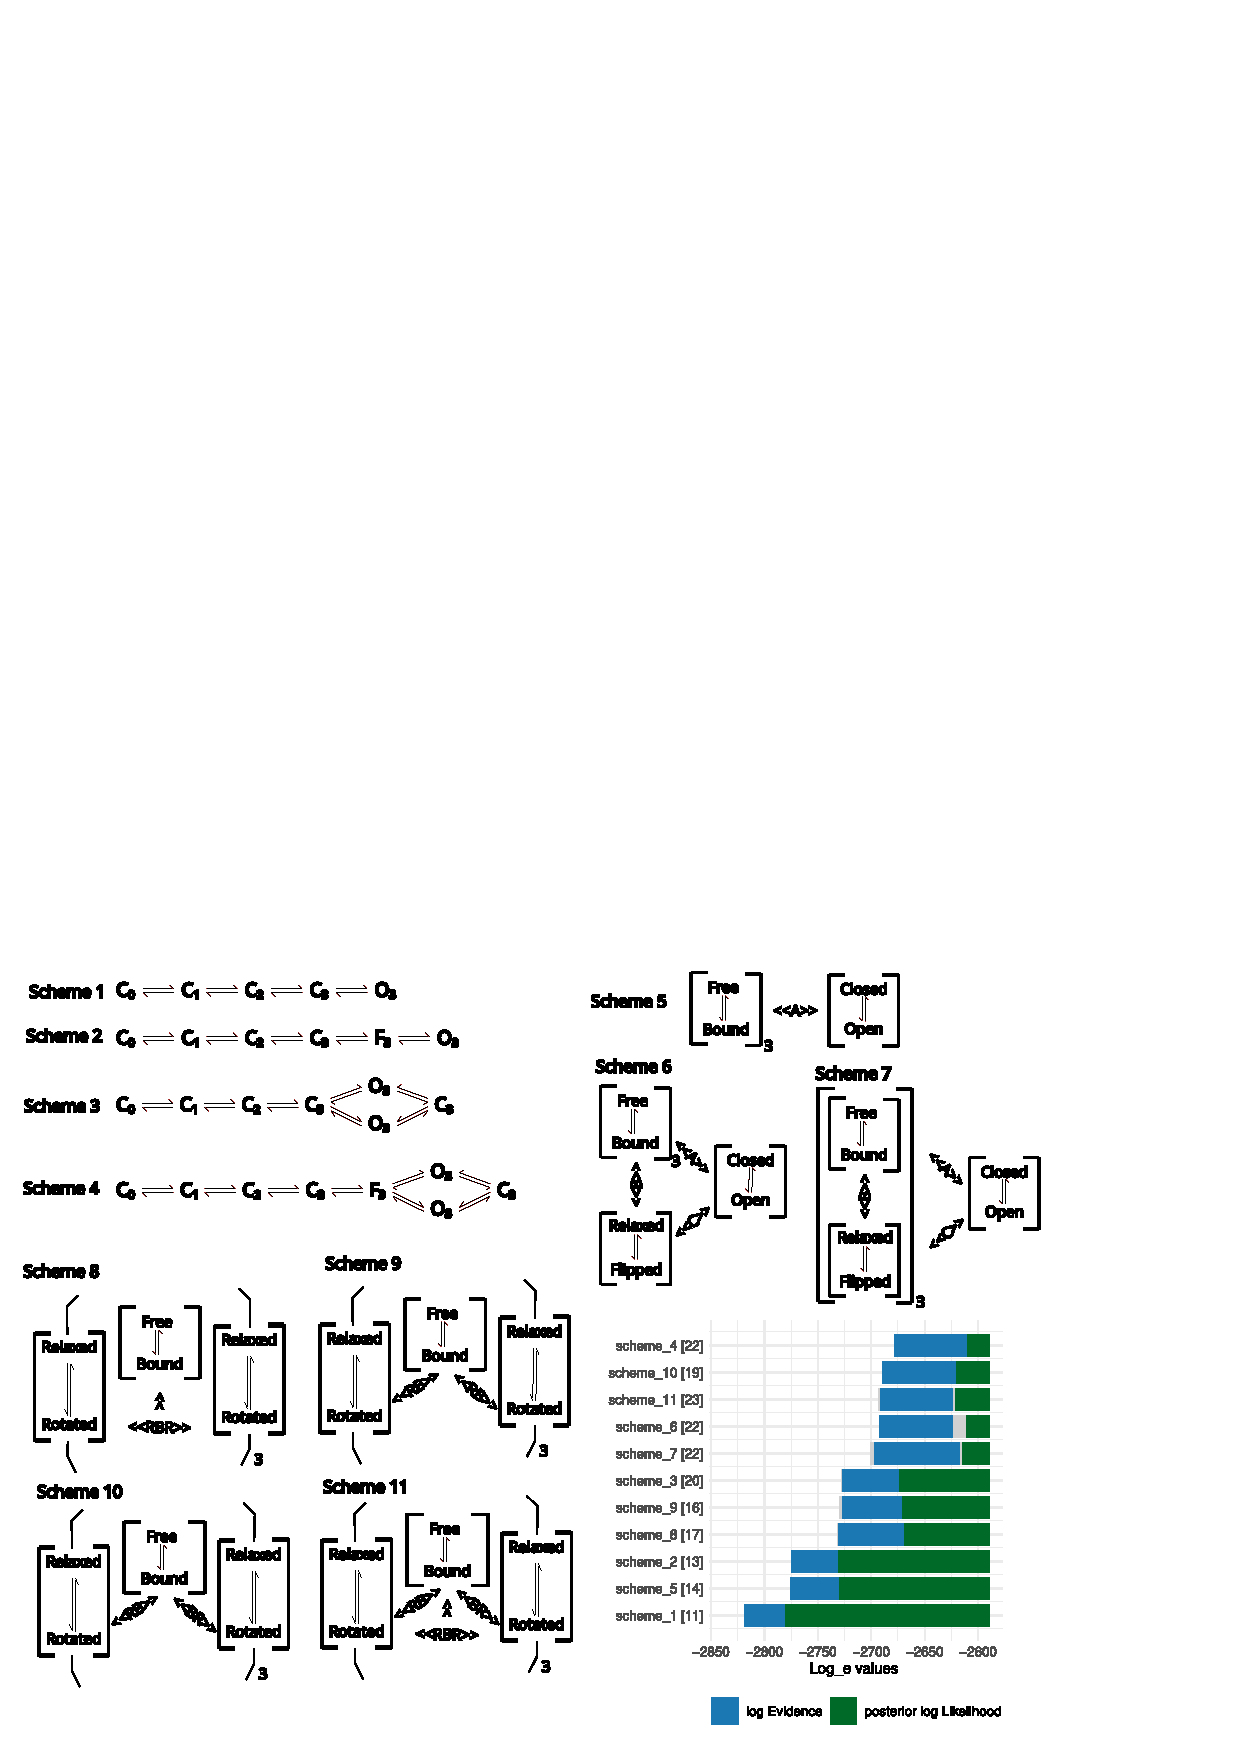
\includegraphics[width=\linewidth]{Figure_1.pdf}
	\caption{\textbf{Bayesian Evidence for Conformational, Allosteric, and State Models.}  
		(\textbf{a}) Schematic representation of the newly proposed conformational models. R: resting; F: flipped; RA: agonist-bound; RB, BR: rotation-binding and binding-rotation allosteric couplings, indicating interactions with the left or right subunit; RBR: rotation-binding-rotation ternary allosteric coupling. Dotted lines indicate repeated segments as specified by the subscript. In Scheme~IX, RB equals BR; in Scheme~X they differ; and in Scheme~XI ternary coupling is also present.  
		(\textbf{b}) State Scheme~IV: C: closed state; CA$_n$: closed state with $n$ agonists bound; F: flipped state; O$_n$: $n$th alternative open state; D: a potentially desensitized closed state with restricted unbinding.  
		(\textbf{c}) Allosteric Schemes~VI and VII: C: closed channel; O: open channel; A, B, C: allosteric couplings; subscripts indicate repetition.  
		(\textbf{d--e}) Bayesian evidence for each illustrated scheme, computed using the recursive MacroIR algorithm (\textbf{d}) and the non-recursive MacroINR algorithm (\textbf{e}). Color coding facilitates comparison of scheme rankings. Gray rectangles denote the standard error of $\log_e(\text{Evidence})$.  
	}
	\label{fig:figure1}
\end{figure}

\begin{extfigure}[t]
	\centering
	\includegraphics[width=\linewidth]{Supplementary_Figure_1.pdf}
	\caption{\textbf{Bayesian Evidence for All Conformational, Allosteric, and State Models.}  
		(\textbf{a}) Schematic representation of the new conformational models. R: resting; F: flipped; RA: agonist-bound; RBR: rotation-binding-rotation ternary allosteric coupling. Dotted lines indicate repeated segments as specified by the subscript.  
		(\textbf{b}) State models (Schemes~I–III): C: closed state; CA$_n$: closed state with $n$ agonists bound; F: flipped state; O$_n$: $n$th alternative open state; D: a potentially desensitized closed state with restricted unbinding.  
		(\textbf{c}) Allosteric Scheme~V: C: closed channel; O: open channel; A: allosteric couplings; subscripts indicate repetition.  
		(\textbf{d--e}) Bayesian evidence for each tested scheme, computed using the recursive MacroIR algorithm (\textbf{d}) and the non-recursive MacroINR algorithm (\textbf{e}). Color coding facilitates comparison of scheme rankings. Gray rectangles denote the standard error of $\log_e(\text{Evidence})$.  
	}
	\label{extfig:1}
\end{extfigure}

\section{Analysis of the Posterior Distribution of Scheme X Parameters}
The posterior distributions of parameters in Kinetic Scheme X (Fig.~\ref{fig:posterior_SchemeX}) reveal three distinct patterns. First, parameters governing kinetic rates, conductance, noise, inactivation constants, and baseline currents exhibit narrow, unimodal distributions, indicating robust identifiability and strong data constraints. The Posterior Concentration Factor (PCF) of these parameters was between 16.9 and 68 (Supplementary Information Table S4), reflecting reduced uncertainty upon incorporating
the data.
Second, two parameters that characterize the relationship between conductance and the number of rotated subunits—namely, the closed-channel leakage and the current-rotation coupling—show modest yet consistent divergence from their priors (PCF of 1.5 and 3, Supplementary Information Table S4). This suggests that while the data constrain these parameters to specific ranges, they do not provide sufficient information to establish a lower bound for the leakage current. Finally, the parameters related to binding-rotation coupling display bimodal distributions, as anticipated given that kinetic data alone cannot resolve the inherent left–right symmetry of the allosteric coupling. Although weakly informative priors were employed to favor one pathway, the affine-invariant ensemble Monte Carlo sampling recovered both modes in proportions consistent with the prior, reflecting this symmetry.
\begin{figure}[t]
	\centering
	\includegraphics[width=\linewidth]{Figure_2.pdf}
	\caption{\textbf{Posterior distributions of model parameters for Scheme X.}  
		(\textbf{a}) Kinetic rate constants: \(r_{\text{on}}\) (rotation), \(r_{\text{off}}\) (return to resting state), and \(b_{\text{off}}\) (unbinding).  
		(\textbf{b}) Association rate: \(b_{\text{on}}\) (binding).  
		(\textbf{c}) Rotation-conductance coupling factor (\(R\gamma\)).  
		(\textbf{d}) Closed-channel leakage ratio (\(\rho_{\text{leak}}\)).  
		(\textbf{e}) Allosteric coupling factor affecting the binding rate (\(BR_{b_{\text{on}}}, RB_{b_{\text{on}}}\)).  
		(\textbf{f}) Single-channel current of the fully rotated channel (\(\gamma\)).  
		(\textbf{g}) Baseline current (\(i_0\)).  
		(\textbf{h}) White noise power (\(\epsilon^2\)).  
		(\textbf{i}) Pink noise power (\(\nu^2\)).  
		(\textbf{j}) Equilibrium allosteric coupling factors (\(BR, RB\)).  
		(\textbf{k}) Allosteric coupling factors affecting the rotation rate (\(BR_{r_{\text{on}}}, RB_{r_{\text{on}}}\)).  
		(\textbf{l}) Number of active channels (\(N_{\text{ch}}\)).  
		(\textbf{m}) Inactivation rate (\(k_{\text{inact}}\)).  
		The gray line represents the prior distribution, while the solid line indicates the posterior distribution. The probability density is normalized to its maximum value for each parameter.
	}
	\label{fig:posterior_SchemeX}
\end{figure}

\textcolor{red}{Aqui es un buen punto para introducir  la Molecular dynamics, ya que la usaríamos para ver cual es RB y cual BR. 
}

\section{Single-Bound P2X Molecular Dynamics Simulations}
To investigate the reasons under the segregation of the binding-rotation coupling into two populations, we examined the initial displacements of the two chains that interact with ATP when this agonist is docked to a single binding site of the closed form of P2X (P2X$^{closed}_{1-ATP}$). For this, we projected onto vectors P2X$^{closed}_A$ $\rightarrow$ P2X$^{open}_A$ and P2X$^{closed}_B$ $\rightarrow$ P2X$^{open}_B$, the  P2X$^{closed}_{1-ATP}$ conformational ensemble computed by means of MD simulations. 
The resulting values were then normalized considering the magnitude of the respective transition vectors, and multiplied by 100 to express them as a percentages for the transition between the closed and open form of the extracellular vestibule (EV). Figure \ref{fig:distri} illustrates the distribution of these values.

\begin{figure} [hbtp!]
  \begin{center}
    \includegraphics[width=0.9\textwidth]{distrib.ab.png}
    \caption{Normalized distribution of the projections of the P2X$^{closed}_{1-ATP}$ conformations sampled during the MD simulations onto P2X$^{closed}_y$$\rightarrow$P2X$^{open}_y$ where y indicates either A or B. Projections were normalized considering the module of the transition vectors and multiplied by 100 in order to express them as percentages.
    Data related to chain A is presented with red while blue is used for chain B. The extracelullar vestibule is highlighted for both chains. The head domain and left flipper of chain A, and the dorsal fin of chain B are also pointed out.}
 \label{fig:distri}
 \end{center}  
\end{figure}

The results demonstrate that ATP binding at the A-B binding site split the conformations of EV of these chains into two populations.
By he one side, it stabilizes the B-chain EV in conformations closely resembling the closed form. In fact this structural analysis reveals that the predominant conformations exhibit minimal deviation, with EV displacements averaging just 3.69\% toward the open-state configuration. Although small, there is a group of conformations that reaches values between 20\%-30\% of the closed-to-open transition range. 
In contrast, results related to the A-chain indicate that the EV region of this monomer is most likely to be found in 20\% of the closed-to-open transition range and that P2X$^{closed}_{1-ATP}$ conformations with values greater than 40\% are still probable. These findings suggest that the perturbation caused by ATP binding to a single site induces asymmetric movements in the chains interacting with the agonist, favoring more the transition of EV toward the open state in chain A that in B one. 
The results are in line with the analysis of the Posterior Distribution of the coupling parameters: there is one coupling that is stronger than the other, and therefore multi-modality arises.  

Using these MD results, we addressed the multimodality of the coupling parameters. We segregated the posterior samples into two subpopulations based on the dominant coupling (RB~$>$~BR or BR~$>$~RB). Based on our MD results, we interpret that the dominant coupling is indeed RB~$>$~BR. In cases where BR~$>$~RB, we swapped the values of (BR, RB), (BR$_{b_{\text{on}}}$, RB$_{b_{\text{on}}}$), and (BR$_{r_{\text{on}}}$, RB$_{r_{\text{on}}}$). This procedure collapsed the bimodal distribution into a unimodal one, ensuring practical identifiability without compromising the model's predictive power. Overall, our approach underscores how mechanistic symmetries can manifest as multimodality in Bayesian inference, necessitating targeted post-sampling analyses that break the symmetry to extract interpretable parameters.

From the perspective of the energetic landscape, the MD simulations suggest that ATP binding promotes a wider exploration along the rotation transition of subunit A compared to subunit B. This indicates that ATP binding may inherently lower the energetic barrier for subunit A rotation, rather than for subunit B. We will explore this possibility in the following section.

\section{Structural Basis of Kinetic Rate Modulation}
\begin{figure}[!htbp]
	\centering
	\includegraphics[width=\linewidth]{Figure_3.pdf}
	\caption{\textbf{From Structure to Kinetic Barrier Modulation.} (a) Cubic schematic illustrating three coupled transitions—agonist (ATP) binding, left subunit rotation, and right subunit rotation—where each vertex represents a distinct receptor state and each edge is labeled with its corresponding kinetic expression. Drawings adapted from \cite{abierta_p2x} underscore the correspondence between the model states and channel structures. Arrows indicate subunit rotations and ATP occupancy. Here, $r_{\text{on}}$ and $r_{\text{off}}$ denote the rotation and unrotation rates, respectively, and $b_{\text{on}}$ and $b_{\text{off}}$ denote the binding and unbinding rates. The terms $RB(BR)_{b(r)_{\text{on(off)}}}$ represent the Rotation–Binding (Binding–Rotation) coupling for binding (rotation) or unbinding (unrotation), while $L$ is the ligand concentration. The posterior distributions for the rate constants of binding and rotation segregate into four clusters that reflect the receptor’s structural states (both subunits resting, left rotated, right rotated, and both rotated for binding; and both binding sites free, right occupied, left occupied, and both occupied for rotation). Colored lines denote the magnitude of the logarithm of the allosteric coupling factors for the \textit{on} and \textit{off} transitions. (d) Log–log plot of the \textit{on} versus \textit{off} rate coupling factors, which captures how ATP binding or subunit rotations differentially accelerate or decelerate the kinetic transitions. Insets illustrate the corresponding changes in the energetic barriers for binding and rotation, computed with a preexponential factor of $10^{-6}$~s (light blue and yellow: BR for binding and rotation; dark blue and red: RB for binding and rotation).}
	\label{fig:rates_SchemeX}
\end{figure}

Our kinetic schemes incorporate two distinct allosteric coupling mechanisms that depend on whether modulation involves the subunit to the left (RB, Rotation–Binding; subunit A in Figure~\ref{fig:distri}) or the subunit to the right (BR, Binding–Rotation; subunit B in Figure~\ref{fig:distri}) of the ATP binding site. Figure~\ref{fig:rates_SchemeX}a illustrates this concept using a cubic schematic of three coupled transitions—agonist binding, left subunit rotation, and right subunit rotation. In this depiction, each vertex represents a distinct receptor state (ranging from unrotated/free/unrotated to rotated/bound/rotated), and each edge is annotated with its corresponding kinetic expression. In the absence of ATP, both subunits rotate at identical rates; however, ATP binding breaks this symmetry, as demonstrated by our MD simulations. Moreover, when both subunits are rotated, the binding and unbinding rates are modulated by the product of the RB and BR couplings.

Traditional allosteric models treat coupling as a single multiplicative factor that alters equilibrium constants. In contrast, our kinetic framework employs two separate factors—one for each conformational change—to capture not only shifts in equilibrium but also modifications of the energetic barriers between states. Each conformational change is governed by its own coupling parameter, allowing for differences in how one conformational change influences the energetic landscape of the other.

Figures~\ref{fig:rates_SchemeX}b and \ref{fig:rates_SchemeX}c show representative posterior distributions (from a 4000-point sample) for the rate constants governing a single binding site (panel b) and a single subunit (panel c). Binding rate constants segregate into four clusters corresponding to distinct structural states---both subunits resting, left rotated, right rotated, and both rotated---while rotation rate constants cluster according to binding site occupancy (unoccupied, right occupied, left occupied, and both occupied). Colored lines indicate the magnitude of the allosteric coupling factors for the \textit{on} and \textit{off} transitions, with the diagonal axes representing log affinity [$\log(b_{\text{off}})-\log(b_{\text{on}})$] or log efficacy [$\log(r_{\text{on}})-\log(r_{\text{off}})$].

The unbinding rate (Figure~\ref{fig:rates_SchemeX}b) is maximal when both subunits are resting, minimal when both subunits are rotated, and assumes intermediate values when only a single subunit is rotated, indicating that $RB_{b_{\text{off}}}\approx BR_{b_{\text{off}}}$. In contrast, the binding rate is maximal when the left subunit is rotated and minimal when the right subunit is rotated, suggesting that $RB_{b_{\text{on}}}\gg1$ and $BR_{b_{\text{on}}}\ll1$. Similarly (Figure~\ref{fig:rates_SchemeX}c), the rotation rate is minimal for unoccupied subunits, slightly higher when the left binding site is occupied, maximal when both sites are occupied, and slightly lower when only the right site is occupied. The unrotation rate varies according to the state of the left site, collectively indicating that $RB_{r_{\text{on}}}\gg1$, $RB_{r_{\text{off}}}\gg1$, while $BR_{r_{\text{on}}}\approx 1+\epsilon$ and $BR_{r_{\text{off}}}\approx 1$. 

These observations reveal a marked asymmetry between the RB and BR couplings. The RB mechanism strongly modulates the equilibrium constants for both affinity and efficacy, whereas the BR effect is comparatively weaker. Moreover, this asymmetry manifests differently when comparing the effect of rotation on binding versus the effect of binding on rotation. In the former, opposite effects on binding are observed; in the latter, both sites are affected similarly, albeit with differing magnitudes.

Figure~\ref{fig:rates_SchemeX}d deepens this insight by plotting the logarithm of the \textit{on} rate coupling against that of the \textit{off} rate. In this log–log representation, a positive \textit{on} log factor indicates that the active state of the allosteric partner accelerates the transition, while a negative value reflects deceleration. Since the equilibrium constant is determined by the ratio of the \textit{on} to the \textit{off} rates, the overall allosteric effect is dictated by the balance between these contributions. Positive allosterism appears when the \textit{on} factor exceeds the \textit{off} factor (i.e., $f_{\text{on}} > f_{\text{off}}$, observed below the diagonal), whereas negative allosterism arises when $f_{\text{on}} < f_{\text{off}}$. If the mechanism solely stabilizes the active state, one expects a highly positive \textit{on} factor coupled with a moderately negative \textit{off} factor; if it destabilizes the resting state, the reverse is true. When both mechanisms contribute, the \textit{on} and \textit{off} factors tend to be of comparable magnitude but opposite in sign---a pattern exemplified by $RB_{b_{\text{on}}}$ (Fig.~\ref{fig:rates_SchemeX}d, dark blue), which robustly stabilizes the bound state while modestly destabilizing the free state.

Importantly, plotting the kinetic coupling factors on a log–log scale enables the classification of positive allosterism into three distinct categories. \textbf{Regular allosterism}---characterized by accelerated \textit{on} rates and reduced \textit{off} rates---appears in the lower right quadrant. \textbf{Catalytic allosterism}, in which both \textit{on} and \textit{off} rates are enhanced (thus lowering the energy barrier), emerges in the upper right quadrant. In contrast, \textbf{inhibitory allosterism}---where both rates are diminished, thereby increasing the energy barrier---is found in the lower left quadrant. This classification provides a clear and visually intuitive framework for understanding the multifaceted nature of allosteric modulation.

The catalytic allosterism observed for the effect of binding on rotation is consistent with the increased amplitude of subunit A movements upon ATP binding, thereby illustrating the correspondence between our MD and kinetic results.
\section{Integrating Subunit Conformational Dynamics into Channel Kinetics}
Building on our model of kinetic coupling at the subunit level, we developed a comprehensive Markov framework to elucidate how molecular interactions collectively govern channel behavior (Fig.~\ref{fig:SchemeX_full}). In our schematic, each subunit is represented as a large ellipse that encapsulates nested binding sites. Resting (unrotated/free) and activated (rotated/bound) conformations are distinguished by empty versus filled ellipses, with rotated subunits drawn in an orientation reflecting activation. Transition dynamics are conveyed via a color code: gray for baseline non-interacting states, orange for strong RB-type interactions, light blue for moderate BR-type interactions, and purple for combined interaction states. Vertical transitions correspond to subunit rotations, whereas horizontal transitions represent ligand binding and unbinding events.

\begin{figure}[!htbp]
	\centering
	\includegraphics[width=\linewidth]{Figure_4.pdf}
	\caption{\textbf{Kinetic Scheme X: A Comprehensive Representation of Subunit Interactions in Channel Activation.} Each subunit is depicted as an ellipse containing nested binding sites; empty ellipses denote resting (unrotated/free) states, and filled ellipses indicate activated (rotated/bound) states. Transition dynamics are color-coded: gray represents baseline non-interacting states; orange indicates strong RB-type interactions; light blue corresponds to moderate BR-type interactions; and purple depicts combined interaction states. Vertical transitions indicate subunit rotations, while horizontal transitions represent ligand binding/unbinding events. The kinetic rate matrix is constructed from rate constants (Fig.~\ref{fig:rates_SchemeX}), scaled by the number of subunits/ binding sites available for the transition.}
	\label{fig:SchemeX_full}
\end{figure}

To construct the kinetic rate matrix, we systematically enumerated all possible state transitions. For each transition, the effective rate is obtained by multiplying the corresponding rate constant (Fig.~\ref{fig:rates_SchemeX}) by the number of subunits undergoing that transition. This method captures both the allosteric coupling among subunits and the combinatorial effects inherent to parallel transition pathways.

\begin{figure}[t]
	\centering
	\includegraphics[width=\linewidth]{Figure_5.pdf}
	\caption{\textbf{State Occupancies and Functional Currents Across Rotational States.} (a) Equilibrium state occupancies measured 60\,s after stimulus clearance reveal that stochastic fluctuations yield measurable pre-activation in the absence of ligand, with ~ 15\%  of channels displaying one rotated subunit, 1.1\%  showing two rotated subunits, and 0.02\%  achieving full rotation. (b) Temporal evolution of state probabilities during ATP stimulation indicates that high-concentration ATP pulses (10\,mM) predominantly drive activation via sequential (edge) transitions (ligand binding followed by rotation), whereas deactivation involves central states with mixed bound/unbound configurations. (c) Distribution of unitary currents across rotational states demonstrates that partial activation is functionally significant; channels with two rotated subunits produce 48\% of maximal current, accounting for the baseline current observed under ligand-free conditions.}
	\label{fig:SchemeX_states}
\end{figure}

Using this framework, we computed the equilibrium state occupancies under resting conditions (60\,s post-stimulus clearance). Notably, stochastic fluctuations produce measurable occupancy in pre-activated states even in the absence of ligand (Fig.~\ref{fig:SchemeX_states}a), a phenomenon quantitatively captured by our MacroIR analysis, which attributes current fluctuations to intrinsic stochastic state transitions rather than measurement noise.

The temporal evolution of state probabilities during ATP stimulation reveals distinct activation and deactivation pathways (Fig.~\ref{fig:SchemeX_states}b). High-concentration ATP pulses (10\,mM) promote activation predominantly via sequential edge transitions (ligand binding followed by rotation), while deactivation proceeds through central states characterized by mixed bound and unbound configurations.

Finally, current distributions across rotational states (Fig.~\ref{fig:SchemeX_states}c) demonstrate that partial activation is functionally significant: channels with two rotated subunits generate 48\% of maximal current. Thus, while full channel activation produces the majority of the current during ATP stimulation, pre-activation currents are largely attributable to channels in partially activated (doubly rotated) states.

These findings resolve a longstanding paradox in purinergic signaling by explaining how only two functional ATP binding sites suffice to trigger channel activation.


\section{From State Dynamics to Predictive Likelihood Modeling}
\label{sec:likelihood}

\begin{figure}[t]
	\centering
	\includegraphics[width=\linewidth]{Figure_6.pdf}
	\caption{\textbf{Predictive likelihood modeling from state dynamics, a posterior predictive check} (a) A sample from the posterior distribution of the predicted macroscopic current (blue) closely matches the measured current (black). (b) The total variance of the predicted current is shown, with insets highlighting the contributions of white (red) and pink (green) noise. At maximum time resolution and over ATP concentrations from 0.2 to 10 mM, white noise dominates during the ATP pulse while pink noise is significant during the pre-pulse period. (c) Comparison of the expected (lines) and observed likelihoods computed using a Normal distribution for each measurement.}
	\label{fig:SchemeX_likelihood}
\end{figure}

MacroIR leverages the state distribution illustrated in Fig. \ref{fig:SchemeX_states}a and \ref{fig:SchemeX_states}b, along with the expected current for each state as shown in Fig. \ref{fig:SchemeX_states}c, to compare the predicted macroscopic current with experimental measurements. As depicted in Fig. \ref{fig:SchemeX_likelihood}a, the sample from the posterior distribution of the predicted current closely aligns with the actual data. 

Moreover, MacroIR computes the total variance of the predicted current (Fig. \ref{fig:SchemeX_likelihood}b) by decomposing the contributions from both white and pink noise. The analysis reveals that, at maximum time resolution and over ATP concentrations ranging from 0.2 to 10 mM, white noise is the predominant source during the ATP pulse, whereas pink noise is more pronounced during the pre-pulse period.

Utilizing the expected current and its variance, the partial log-likelihood for each measurement is determined using a Normal distribution. Figure \ref{fig:SchemeX_likelihood}c illustrates a comparison between the expected (lines) and observed likelihoods, thereby validating the model's accuracy.

\section{Discussion}
Our study bridges the longstanding gap between equilibrium-based allosteric models and phenomenological kinetic schemes by introducing a conformational kinetic framework that directly links discrete structural transitions to macroscopic channel function. By leveraging the MacroIR algorithm alongside detailed conformational modeling, we resolved multiple time constants associated with specific structural rearrangements during P2X2 receptor activation. This approach not only captures the evolution of state probabilities but also elucidates the relationship between partial activation and pore opening.

Our findings demonstrate that ATP binding induces an asymmetric conformational response among receptor subunits. Rather than triggering a uniform, concerted transition, ATP binding selectively lowers the energetic barrier for rotation in one subunit while leaving that of its neighbor largely unaltered. Moreover, the rotation of this favored subunit subsequently elevates the energetic barrier for ATP binding at an adjacent site, providing a mechanistic basis for the negative cooperativity observed in previous studies~\cite{Sattler2020UnravellingTI}.

We identified the subunit with the reduced energetic barrier for rotation by analyzing single-bound P2X MD simulations. These simulations revealed a striking asymmetry in fluctuations along the rotation axis between the two chains forming the binding site. While chain B, on the right side of the binding site, exhibits only minor movements, chain A, on the left, shows considerably larger displacements, consistent with a lowered energetic barrier for rotation.

Although the activation kinetic profile could, in principle, be achieved without barrier modulation by assuming higher basal turnover rates, the differential modulation we observed suggests an increased energy barrier for resting-state rotation. This elevated barrier limits the time the channel spends in transitional conformations in the absence of an agonist, likely reducing the risk of spontaneous inactivation. Conversely, a reduction in both rotation and unrotation rates prolongs the time constant of unliganded gating noise, rendering it detectable by our analysis.

Mitigating risk by raising the energetic barrier in the inactive state appears to be a prudent strategy, leading us to propose that this mechanism constitutes a fundamental design principle in protein kinetics. By elevating the energy barriers for non-productive transitions, the receptor minimizes high-risk conformations. This strategy not only preserves protein functionality but also ensures rapid, ligand-induced responses when necessary. Overall, this mechanism, which fine-tunes transition frequency rather than merely shifting equilibrium populations, may represent a general strategy by which dynamic proteins balance functional responsiveness with resilience.

The flip state was initially proposed for glycine receptors~\cite{burzomato2004single} and later extended to purinergic receptors~\cite{Moffatt_hume, jiang2012intermediate, browne2013p2x}. Here, we show that a model based on subunit rotation, rather than invoking a discrete flip state, can explain the same experimental data that originally motivated the flip state hypothesis for P2X2 receptors.

Beyond its mechanistic implications, our work has significant methodological and translational ramifications. The MacroIR framework provides a powerful tool for extracting kinetic information from time-averaged macroscopic currents, and its integration with structural data paves the way for a new era of dynamic structural biology. From a therapeutic standpoint, targeting kinetic couplings rather than equilibrium constants may yield next-generation modulators with improved specificity for conditions such as chronic pain and inflammation.

In summary, by unifying structural dynamics with kinetic principles, our study redefines allosteric regulation as an evolutionarily optimized modulation of transition pathways rather than mere state stabilization. This kinetic-conformational paradigm not only resolves long-standing discrepancies between structural snapshots and functional measurements but also opens new avenues for protein engineering and targeted drug design.

\bibliography{biblio}% common bib file

\end{document}
